\documentclass[a4paper,11pt,phdthesis,singlespace,twoside]{cssethesis}

\usepackage{harvard} % Use the Harvard bibliography and citation package
\usepackage{graphicx}
\usepackage{epstopdf}
\usepackage{mathptmx}
\usepackage{times}

\usepackage{algorithm}
\usepackage{enumitem}
\usepackage{listings}
\usepackage{color}
\usepackage{apacite}
\usepackage{multirow}

\thesisauthor{Viet Vo}
\thesisauthorpreviousdegrees{BSc., MSc.}
\thesisdepartment{Caulfield School of Information Technology}
\thesisauthorstudentid{26356988} % Needed for litreview
\thesisauthoremail{viet.vo\@@monash.edu} 

%\thesismonth{October} % Optional. Current month is used if this is not set
%\thesisyear{2015} % Optional. Current year is used if this is not set
\thesistitle{The Effects of Group Member's Parameters on Human Crowd Modelling}
\thesissupervisor{Prof. Bernd Meyer}
\thesissupervisoremail{bernd.meyer\@@monash.edu} 
\thesisassocsupervisor{Dr. Aldeida Aleti} 
\thesisassocsupervisoremail{aldeida.aleti\@@monash.edu} 
%\thesisdedication{}
% start the document
\begin{document}

\frontmatter					% start the thesis front matter.

\thesistitlepage				% Generate the title page.
%\thesiscopyrightpage			% Generate the copyright page.
%\thesisdedicationpage			% Generate a dedication page (optional)
\tableofcontents				% Generate a table of contents.
\listoftables					% Generate a list of tables (optional).
\listoffigures					% Generate a list of figures (optional).

\begin{thesisabstract}			% generate the abstract page.
Nowadays, rapid urbanization and population growth becomes inevitable challenges in the effort of planning infrastructure, estimating traffic needs and capacities, and increasing the safety of pedestrians. To develop realistic simulation models, various studies have been conducted in order to understand and simulate behaviors which can emerge in both normal and emergency situations such as groups of pedestrians moving with or competing against each other. These models mainly investigate how model's outputs which are group's formation, cohesion degree, and speed change when group population size varies, or explore the collective behavior of flocking organisms at randomly chosen values of model's parameters. However, they have not yet investigated systematically the effect of model's input parameters to explore the most influential parameters which control group information, and how group cohesion affect individuals to make them maintain group cohesion. Yet, the impact of group cohesion behavior caused by model's parameters on flow rate which is a crucial measurement of crowd modelling also has not been studied in previous studies. Therefore, this PhD study aims to resolve this research question by using systematic analysis methods and proposed simulation scenarios when considering group of pedestrians is the collection of members who have the same scalar parameter value or different parameter distributions. This work is to advance our knowledge about the role of model's parameters for improving real-time prediction systems and calibration works based on these models.

\end{thesisabstract}                 
\let\cleardoublepage\clearpage
%\thesisdeclarationpage			% generate the declaration page (optional).

%\begin{thesisacknowledgments}	% generate the acknowledgements page (optional).
%I would like to thank everyone who helped to make this possible. It has
%been an incredible journey of self-discovery, and I love every last one of
%you\ldots
%\end{thesisacknowledgments}   

%%%%%%%%%%%%%%%%%%%%%%%%%%%%%%%%%%%%%%%%%%%%%%%%%%%%%%%%%%%%%%%%%%%%%%%%%%%%%%
%%
%% Main matter 
%%
\mainmatter						% start the thesis body.

\chapter{Introduction}
\let\cleardoublepage\clearpage
Since over 70\% of the world population is predicted to live in cities by 2050 \cite{Weidmann2012}, rapid urbanization and population growth will be inevitable challenges in the effort of planning infrastructure, estimating traffic needs and capacities, and increasing the safety of pedestrians. With the increase in the number of public events and the number of accidents during these events since the crush disaster happened at the Station Nightclub, USA (2003) \cite{Evers2011}, the demand for realistic crowd simulation models becomes important for risk management in urban design and crowd safety. To develop realistic simulation models, various studies have been conducted in order to understand and simulate behaviors which can emerge in both normal and emergency situations such as groups of pedestrians moving with or competing against each other.

Group cohesion behaviour is the behaviour of objects moving towards the average positions of their neighbors over the time \cite{Reynolds1987}. The definition of this behaviour was motivated by the visual observation of coherently flying objects. The behaviour has been investigated widely on the collective motion of different flocking organisms including homing pigeon flocks \cite{Kattas2012}, fish schools \cite{Miller2013}, and bacteria colony \cite{Cisneros2007}. 

Human group cohesion behaviour is observed by its cohesion degree and formation. Cohesion degree denotes the average distance to the group’s centre of mass from each group member while observable human group formations are V-like, line-abreast, U-like, or river-like \cite {Helbing2005}. Group cohesion behaviour is important in both normal and evacuation scenarios. In normal situations, group cohesion behaviour can affect the speed and movement direction of pedestrians who are not belonging to any group. In human behaviour research, the frequency of group cohesion behaviour’s occurrence has been observed at different places in the UK with the percentages of 37\% at train station, 50\% at shopping centre, 28\% at university campus, 50\%, at Clumber Street \cite{Singh2009}. Pedestrians in the same group might be family members, colleagues. In crowd disasters, pedestrians evacuate with group rather than escape individually. Groups of families and friends with strong ties, stay together and evacuate together have been emphasized through socio-psychological research area \cite {Mawson2005}. They may move irrationally to maintain its cohesion and consequently become obstacles for other pedestrians \cite{Aguirre2011}.

Various models have been constructed to understand group cohesion behaviour such as the cellular automata model, the social-force based model, the standard Vicsek model. These models mainly investigate how model’s outputs which are group’s formation, cohesion degree, and speed change when group population size varies, or explore the collective behaviour of flocking organisms at randomly chosen values of model’s parameters. However, they have not investigate systematically model’s input parameters to explore the most influential parameters which control group information, and how group cohesion affect individuals to make them maintain group cohesion. Yet, the impact of group cohesion behaviour caused by model’s parameters on flow rate which is a crucial measurement of crowd modelling also has not been studied in current studies. Therefore, this PhD study aims to resolve these two research gaps by using systematic analysis methods and proposed simulation scenarios when considering group is the collection of members have the same scalar parameter value or different parameter distributions. This work is to advance our knowledge about model’s the most influential parameters for improving real-time prediction systems and calibration works based on these models, and the impact of group cohesion on flow rate measurement for predicting empty and occupied space for evacuation plan.

Chapter 2 of this report represents the state of the art from models trying to understand group cohesion behaviour. Chapter 3 analyses the drawbacks of current models and presents the need of this research study through proposed research questions. Chapter 4 presents research methodology to resolve these questions. Chapter 5 reports the contribution of this study. Chapter 6 reports current working progress and research timeline to answer these questions. Finally, Chapter 7 outlines compulsory research training hours undertaken in the IT faculty.

\chapter{Literature Review}
\let\cleardoublepage\clearpage
This chapter reviews current models that have been constructed to understand group cohesion behaviour. Modelling approaches are various from modelling the changes of each cell on a grid layout, investigating social forces that affect each pedestrian’s acceleration, to providing standard Vicsek model which has been applied widely in flocking organisms with fewer parameters to simulate group members.

\section{Cellular automata model for group behaviour}
Cellular automata-based group behaviour model is the approach relying on Von Neumann's idea that divides space into uniform grid or hexagonal cells. At each time \textit{t}, variables at each cell are updated according to a set of local rules or its neighbour cells. Common local rules are moving direction, or avoidance rules. Every cell in the space can be in different states including free, an obstacle, or occupied by a pedestrian. General cellular automate model is formed as formulas (2.1-2.3).
\begin{equation}
Env = c_{0},c_{1},c_{2},c_{3,},\ldots where\/ \forall c_{i} \in \tetit{Cell}
\end{equation}
\begin{equation}
neighbours(c) = {(c),S(c),E(c),W(c),NE(c),SE (c),NW(c),SW(c)}
\end{equation}
\begin{equation}
State(c)= s \in \left \{Free,Obstacle,Pedestrian_{i}\right \}
\end{equation}
Every cell has variables of path field, obstacle field, and density field. Path field is to identify distance from current cell to destination cell. Obstacle field indicates for every cell the distance from an obstacle or a wall. Density field is to indicate for each cell the crowd density in the surroundings at the current time step t. When running a CA-based pedestrian model, there is several update strategies including parallel update, sequential update, or shuffled sequential update. 

To simulate group behaviour, \cite{Bandini:2011} constructed pedestrians on these defined cells. A pedestrian is represented as a utility-based agent having following attributes:
\begin{equation}
Pedestrian: (Id,GroupId,State,Actions,Destination)
\end{equation}
where:
\begin{itemize}
  \item Id\textendash identification number of pedestrian \textit{i}
  \item GroupId\textendash identification number of group that pedestrian \textit{i} belongs to
  \item State\textendash represents pedestrian's current cell that and direction followed in last movement
	\item Actions\textendash the set of possible actions to choose an appropriate cell from equations (2.5) and (2.3)
	\item Destination\textendash reflects current path field of the cell where pedestrian i is in
\end{itemize}
An utility function \begin{math}U_{t}(c)\end{math}  was proposed by the author as in equation (2.5). The function estimates the probability of cell \textit{c} to allow pedestrian \textit{i} move in to maintain group cohesion at each time step \textit{t}.
\begin{equation}
U_{t}(c)= \frac{k_{g}G(c)+k_{ob}Ob(c)+k_{s}S(c)+k_{d}D(c)+k_{ov}Ov(c)+k_{c}C_{i}(c)+k_{i}I_{i}(c)}{d}
\end{equation}
where:
\begin{itemize}
  \item $ \begin{math} \textit{k_{g}}, \textit{k_{ob}}, \textit{k_{s}},\textit{k_{d}},\textit{k_{ov}},\textit{k_{c}},\textit{k_{i}}  \in [0,100] \end{math} $ are model's parameters for their corresponding functions 
	\item  \begin{math} G(c)\end{math} is the goal attraction derived from current cell's path field and destination cell's path field 
	\item  \begin{math} Ob(c)\end{math} represents obstacle repulsion from obstacle field of current cell c over the maximum distance to obstacles from any cell in grid layout 
	\item  \begin{math}S(c)\end{math} represents separation value to allow pedestrian i avoid other pedestrians. It is measured by density field of current cell c over the predefined maximum density 
	\item \begin{math}D(c)\end{math} represents whether this cell is the same direction with previous movement of pedestrian 
	\item \begin{math}Ov(c)\end{math} represents a small probability to allow two pedestrians stay on the same cell
	\item \begin{math}C_{i}(c)\end{math} represents cohesion value of cell \textit{c} if pedestrian \textit{i} move in towards other group member's position
	\item \begin{math}I_{i}(c)\end{math} is used in the case of large group which can be separated into sub groups. It represents the cohesion value of current pedestrian toward the largest group
	\item \textit{i} is the distance from cell \textit{c} to pedestrian \textit{i}'s current cell position. d is only equal to 1 or \begin{math} \sqrt{2} \end{math}
\end{itemize}	
Group cohesion degree is then defined as in equation (2.6) to represent the average distance from each group member to group's centre of mass. The study used this degree to support pedestrian \textit{i} trade off current goal attraction with group cohesion based on predefined rules.
\begin{equation}
Cohesion(Group)= \frac{\sum_{\substack{i=1}}^{Size(Group)}distance(centroid,a_{i})}{Size(group)}
\end{equation}
The study then measured the correlation between group size and group cohesion speed in various design layouts. However, this CA-based model only allows pedestrians move in neighbour cells rather than in further cells at each time step. It applied the same value of each parameter \begin{math} \textit{k_{g}}, \textit{k_{ob}}, \textit{k_{s}},\textit{k_{d}},\textit{k_{ov}},\textit{k_{c}},\textit{k_{i}}  \in [0,100] \end{math} for whole group members. Group speed and cohesion degree are investigated when group population size varies; specifically, group speed decreases when increasing population size. However, the effect of these parameters on group degree and the impact of group cohesion behaviour on flow rate measurement were not investigated by its authors.

\section{Social force model for group behaviour}
Moussaid, Helbing and colleagues \cite{Moussaid2010} created the social group-force model based on the social-force model \cite{Helbing1995} \cite{Helbing2000}. The social group model (equation 2.7-2.8) represents that a pedestrian \textit{p} at time \textit{t} is trying to move with a certain desired speed \begin{math} \textit{v_{p}^{d}(t)} \end{math} in a desired direction \begin{math} \textit{\vec{e}_{p}^{\,d}(t)}\end{math} pointing from pedestrian \textit{p}'s current position to his target position . Therefore, pedestrian \textit{p} tends to correspondingly adapt his actual velocity \textit{\vec{v}_{p}(t)}\end{math} with a certain acceleration time \begin{math}  \tau_{p} \end{math}. The acceleration time represents pedestrian \textit{p} changes its current velocity and return to its desired velocity. Pedestrian \textit{p}'s acceleration at time \textit{t} is also influenced by repulsive forces coming from surrounding pedestrians and obstacles. They are \begin{math} \sum_{\substack{\textit{q}\neq(\textit{p})}}\vec{f}_{\textit{pq}}(\textit{t}) \end{math} and \begin{math} \sum_{\gamma}\vec{f}_{\textit{p\gamma}}\end{math} (\textit{t})  respectively. The repulsive force’s directions and group force direction are represented in Figure~\ref{fig:repulsive_force}. The group influence force \begin{math} \vec{f}_{p}^{group}(t)\end{math} aims to describe that an individual in group continuously adjusts its position to reduce its head direction and maintain group's centre of mass, but also avoid other group members. The group force is represented in equation 2.9.
\begin{equation}
\frac{d\vec{v}_{p}(t)}{dt}= \vec{f}_{p}(t) + \xi_{p}(t)
\end{equation}
\begin{equation}
\vec{f}_{p}(t)= \frac{1}{\tau}_{p}}\left(v_{p}(t)\vec{e}_{p}^{\,d}(t) - \vec{v}_{p}(t) \right) + \sum_{\substack{\textit{q}\neq(\textit{p})}}\vec{f}_{\textit{pq}}(\textit{t}) + \sum_{\gamma}\vec{f}_{\textit{p$\gamma$}}(t) + \vec{f}_{p}^{group}(t)
\end{equation}
where \begin{math} \textit{v_{p}^{d}(t)} \end{math} is the desired speed of pedestrian p that varies over time, \begin{math} \xi_{p}(t)\end{math} is an uncertainty factor. 
\begin{equation}
\vec{f}_{p}^{group}(t)= \vec{f}_{p}^{vis}(t) + \vec{f}_{p}^{att}(t) + \vec{f}_{p}^{rep}(t)
\end{equation}
\begin{figure}[ht]
\begin{center}
\resizebox{100mm}{!}{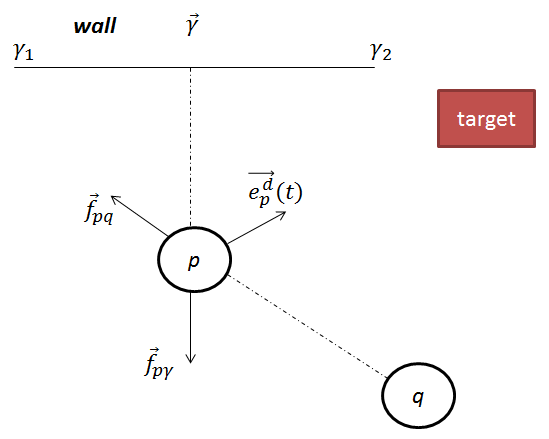
\includegraphics[width=0.05\columnwidth]{figs/repulsive_force.png}}
\end{center}
\caption{Repulsive forces \begin{math}\vec{f}_{\textit{pq}} \end{math} and \begin{math}\vec{f}_{\textit{p$\gamma$}} \end{math} on pedestrian \textit{p} created by pedestrian \textit{q} and wall \gamma}
\label{fig:repulsive_force}
\end{figure}	
The social group force \begin{math}\vec{f}_{p}^{group}(t) \end{math}describes that pedestrian \textit{p} at time \textit{t} turns his gazing direction to see their partners. Thus, \begin{math} \vec{f}_{p}^{vis}(t)\end{math} vision force is included to help pedestrian \textit{p} adjust its position to reduce the head rotation. At the same time, pedestrian \textit{p} keeps a certain distance to the group's centre of mass by the force \begin{math}\vec{f}_{p}^{att}(t)\end{math}. A repulsive force\begin{math} \vec{f}_{p}^{rep}(t)\end{math} is added to support pedestrian \textit{p} avoid other group members. These group element forces are presented in equations (2.10-2.12).
\begin{equation}
\vec{f}_{p}^{vis}(t) = -\beta_{1}\alpha_{p}\vec{V}_{p}(t)
\end{equation}
\begin{equation}
\vec{f}_{p}^{att}(t) = -q_{A}\beta_{2}\vec{U}_{p}(t)
\end{equation}
\begin{equation}
\vec{f}_{p}^{rep}(t) = \sum{\substack{k}}q_{R}\beta_{3}\vec{W}_{pk}(t)
\end{equation}
where:
\begin{itemize}
  \item $\beta_{1}$ is the model's parameter describing the strength of the social interactions between group members
	\item $\alpha_{p}$ is the angle constructed by the vector pointing to target direction and current gazing direction. The angle varies from 0 degree to maximum angel constructed by the target direction and the vector point from pedestrians \textit{p}'s current position to group centre of mass at time \textit{t}. The larger angel $\alpha_{p}$ means that pedestrian \textit{p} feels less comfortable to move and consequently reduce his speed at time \textit{t}. The angle $\alpha_{p}$ is represented in Figure~\ref{fig:alpha_vision}.
\begin{figure}[ht]
\begin{center}
\resizebox{60mm}{!}{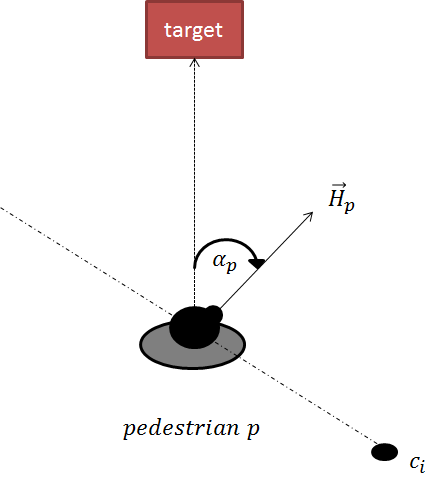
\includegraphics[width=0.05\columnwidth]{figs/alpha_vision.png}}
\end{center}
\caption{Pedestrian \textit{p} turns his gazing direction \begin{math}\vec{H}_{p}(t) \end{math} by an angel \begin{math} \alpha_{p} \end{math} to see group centre c_{i}}
\label{fig:alpha_vision}
\end{figure}	
	\item $\beta_{2}$ is model's parameter describing the strength of the attraction effects
	\item  \begin{math}\vec{U}_{p} \end{math} is the unit vector pointing from pedestrian p to the centre of mass
	\item $q_{A}=1$ if the distance between pedestrian p and group centre of mass exceeds the threshold \begin{math}\frac{N-1}{2} \end{math} meters
	\item $\beta_{3}$ is the model's parameter describing the repulsion strength between group members
	\item $q_{R} = 1$ if pedestrians \textit{p} and \textit{k} overlap each other; otherwise, $q_{R} = 0$
	\item \begin{math}\vec{W}_{pk}\end{math} is the unit vector pointing from pedestrian \textit{i} to the group member \textit{k} 
\end{itemize}	
To summary, the social force model comprises parameters that need to be set at initial simulation time as in Table~\ref{tab:model_params}.

\begin{table}[H]
\caption{Social-group force model's parameters}
\begin{tabular}{|l|l|l|} \hline
\textbf{Parameter} & \textbf{Component} & \textbf{Description} \\ \hline
$ V_{p}^{Id}$ &Desired Acceleration& Initial desired velocity \\ \hline
$ \tau_{p}$ &Desired Acceleration& Acceleration time \\ \hline
$\texit{c}$ &Desired Acceleration& Constant to find maximum velocity  \\ \hline
$ \textit{A}$ & Repulsive Force with other pedestrians& Interaction strength \\ \hline
$ \textit{B}$ & Repulsive Force with other pedestrians& Interaction range \\ \hline
$ \textit{U}$ & Obstacle Force & Obstacle interaction strength  \\ \hline 
$ \textit{R_{p}}$ &  Simulation & Radii of pedestrian \textit{p}\\ \hline 
$ \beta_{1}$ &  Group vision force & The strength of the social interactions\\ \hline 
$ \beta_{2}$ &  Group attraction force & The strength of the attraction effects \\ \hline 
$ \beta_{3}$ &  Group repulsion force & The repulsion strength between group members\\ \hline 
\end{tabular}
\label{tab:model_params}
\end{table}
Social-force based model has possessed a long-life modification period by its author and colleagues for more than a decade in order for simulating the additional factors affecting individual's acceleration or being easier towards calibration process. However, it almost uses the same parameter distribution to simulate pedestrians inside crowd as in Table~\ref{tab:model_params_values}.
\begin{table}[H]
\caption{Social-group force model's parameter values}
\begin{center}
\begin{tabular}{|l|l|l|} \hline
\textbf{Parameter} & \textbf{Value} & \textbf{Reference} \\ \hline
\multirow{2}{*}{$ V_{p}^{Id}(m/s)$}& avg. = 1.34, st. dev. = 0.26 & \cite{Helbing1995}\\ 
															& avg. = 1.3, st. dev. = 0.3 & \cite{Helbing2005} \\ \hline
\multirow{2}{*}{$ \gamma(s)$}& 0.5 & \cite{Helbing1995}\\ 
															& 0.1 & \cite{Helbing2000} \cite{Helbing2005}\\ \hline
\textit{c}&1.3&\cite{Helbing1995} \cite{Helbing2000} \\ \hline
\textit{A}(m/s^{2})&3.0 &\cite{Helbing2005}\\ \hline
\textit{B}(m)&0.2&\cite{Helbing2005}\\ \hline	 																										
\end{tabular}
\end{center}
\label{tab:model_params_values}
\end{table}
Through actual observation, Moussaid found that pedestrians in the same group likely move in a line-abreast formation to allow them communicate with each other easily. When crowd density increases, group of pedestrians automatically change its formation into V-shaped or river-like pattern. According to the study, when the model parameter $\beta_{1}=0$, it shows that group members only try to stick together with no communication rule. When $\beta_{1}=4$, a V-shaped structure is created. 

The authors applied the same value of each parameter in Table~\ref{tab:model_params_values} and parameters of group force $\beta_{1}, \beta_{2}, \beta_{3}$ to all pedestrians inside group to see these patterns. In fact, human group formation is various from V-line, U-like, line-abreast, to river-abreast as in actual observation (Helbing, 2005). However, this model did not mention at which values of parameters $\beta_{1}, \beta_{2}, \beta_{3}$ other group formations could be created. It also raises a question whether these parameters have to be the same for all group members to establish these structures. Similar with CA-based model, the authors of social-group force models have not investigated the effect of member’s parameters (e.g. $ V_{p}^{Id}, \gamma, \textit{A}, \textit{B} $) on group speed and formation. They only studied how these information change according to different group population sizes; specifically, they found that group speed decreases when group population size increases. 

\section{Standard Vicsek model of flocking organisms}
In order to interpret the behaviour of huge flocks of living organisms (flock of birds, fish schools, and bacterium, and human crowd) in the presence of perturbations, a statistical physic approach has been introduced to the flocking by Vicsek \cite{Vicsek1995}. Nowadays, it has been called as Standard Vicsek Model as suggestion of \cite{Huepe2008}. The model considers that self-propelled particles represent living flocks, and perturbations are natural consequence of stochastic and deterministic factors affecting the motion of particle. The model is presented in equations (2.13-2.14).
\begin{equation}
\vec{v}(t+1)= \vec{v}_{0}\frac{\langle\vec{v}_{j}(t)\rangle_{R}}{|\langle\vec{v}_{j}(t)\rangle_{R}|} + \textit{perturbations}
\end{equation}
\begin{equation}
\vec{x}(t+1)= \vec{x}(t) + \vec{v}(t+1)
\end{equation}
The main idea of the model is that at each given time step \textit{t}, particle \textit{i} is usually controlled by interactions with its local neighbors in a constant radius \textit{R} and uncertainty factor perturbations. Here \begin{math}\langle\vec{v}_{j}(t)\rangle_{R} \end{math} denotes the averaging of the velocities of neighbours in radius \textit{R}. The expression \begin{math} \frac{\langle\vec{v}_{j}(t)\rangle_{R}}{|\langle\vec{v}_{j}(t)\rangle_{R}|}\end{math} provides a unit vector pointing in the average direction of motion. The particle \textit{i} also has a constant velocity \begin{math} \vec{v}_{0} \end{math}. In the standard version of the model, Vicsek derived the perturbations factor by adding a random angle to the angle corresponding to the average motion direction of particle \textit{i}'s neighborhood. The angel \begin{math} \vartheta_{i} \end{math} of average motion direction and random angle $\Delta_{i}$ at time \textit{t} are represented as in equations (2.15-2.16).
\begin{equation}
\vartheta_{i}(t)= \tanh\left(\frac{\langle v_{j,x}\rangle_{R}}{\langle v_{j,y}\rangle_{R}}\right)
\end{equation}
\begin{equation}
\vartheta_{i}(t+1)= \vartheta_{i}(t) + \Delta_{i}(t)
\end{equation}
where \begin{math}  v_{j,x} and  v_{j,y} \end{math} are the x and y coordinates of particle \begin{math} \textit{j^{th}}'s \end{math}velocity in the neighborhood of particle \textit{i}. The perturbation $\Delta_{i}(t)$ s a random number taken from uniform distribution in the interval $[-\eta\pi,\eta\pi ]$. The randomness of perturbation makes particles have different motion direction from those of others. The velocity $ \begin{math} \textit{v_{0}} \end{math} $ was set the same for all birds in flocks. Finally, two control parameters of the model are the density $ \rho $ (number of particles in a volume $ \begin{math} \textit{R^{d}} ( \textit{d}  \end{math}$  is the dimension)), and the level of perturbation $\begin{math} \eta \end{math} $.

In the studies of the authors \cite{Vicsek1995}\cite{Czirok2000}, the average momentum of the particles \begin{math}\phi \equiv \frac{1}{N}|\sum_{j}\vec{v}_{j}| \end{math} and the correlation between particles' velocity directions were investigated when varying model's parameters including the level of perturbation, the density $ \rho $ , and population size. In these studies, the author considered the density ρ at the values 2, 4, 0.5 and explored the average momentum at corresponding values of the level of perturbation $\eta$ at 1,2,3,4,5. The author found that the average momentum decreases when decreasing the density or increasing the level of perturbation. 

There is also another approach from the author to investigate the role of model's parameters \cite{Bhattacharya2010} on group cohesion behaviour. This study derived the model in 3D dimensional environment to explore the cohesiveness through the process of landing of bird flocks performing foraging flights. The study explored the heterogeneity in attributes such as the ages, sex, and social status of animals in group or the differences in the perception of external stimuli by assigning to each bird $ \textit{i} $  an inherent switching time $\begin{math} \textit{t_{i}} \end{math}$, such that if the bird begins a flight at time $ \textit{t}=0 $, it would decide to land at time  $ \begin{math}\textit{t}= \textit{t_{i}} \end{math}$.This work was to show that the difference in the attributes implied the difference in energy reserve to maintain an altitude.\begin{math} \text{t_{i}}'s \end{math} was selected from a Gaussian distribution with a given standard deviation $\sigma_{0}$. The study then investigated quantitatively the fraction of birds not landed yet as time $ \textit{t} $ progresses when setting to different \begin{math}\sigma_{0} \end{math} values. However, the model's parameters $\begin{math}\rho ,\eta, \textit{v_{0}} \end{math}$ were set the same for all birds $ \begin{math}(\rho = 2.0, \eta=0.2, \textit{R}=2.0, \textit{v_{0}}= 0.01) \end{math}$.

In summary, standard Vicsek model used the particle-based approach to understand flocking organisms. The author's proposed studies investigated collective behaviour when varying model's parameters arbitrarily, adding a new constraint for landing period of individual group members to simulate the heterogeneity of group members. However, these studies have not yet explored systematically the effect of parameters to find the most influential parameters on collective behaviour. Moreover, these studies also have not yet considered flock of individual group members who have different parameter distributions to those of others in these parameters.

\chapter{Motivation and Research Questions}
\let\cleardoublepage\clearpage
\section{Problem Statement}
Modelling human group cohesion behaviour is important since it represents the effect of groups on flow rate measurement and the change of group’s space occupation. Through the literature review in Chapter 2, understanding group cohesion behavior is mainly performed by three models including the cellular automata-based model, the force-based model, and the standard Vicsek model. 

The CA-based and force-based models almost investigate model's outputs which are group's speed, formation and group cohesion degree when group population size varies. They found that group's speed decreases linearly when group population size increases. However, they have not yet explored the effect of member's parameters on the model's outputs. The most related work to the understanding that effect is Vicsek's studies. Standard Vicsek model relies on particle-based approach to simulate the cohesiveness of flocking organisms. Vicsek and colleagues explore the average direction of flocks and velocity correlation of group members when model's control parameters (interaction radius, random noise constraint) are varied at randomly chosen values of the parameter pair of $ \rho,\eta $. However, they also have not yet explored systematically the most influential parameters which control group behavior, and how group cohesion varies according to the interaction effect of these parameters. Moreover, the effect of group cohesion behavior on individuals and flow rates also have not been investigated in current group cohesion models when group members maintain their cohesiveness. Flow rate is an important observation measure for human crowd modelling since it is used to assess design layouts and evacuation strategies in simulation environments \cite{Cheng2014}.

To summary, the impact of group member's initial parameters on group cohesion model's outputs and the impact of group cohesion behavior on flow rate have not been investigated. Understanding the role of parameters in these models and possible group behavior can be occurred by parameter values are important for crowd modeling to improve calibration process and real-time prediction’s performance respectively. They also enable live-event organizers understand the change of flow rates and occupied space according to group cohesion behavior. 

Exploring the impact of group member’s parameters should consider group members have either the same scalar parameter values as previous studies have performed or different parameter distributions to those of others. In fact, an actual group contains different members in age (children $ \leq 14 $ years old, adults, elders $ \geq 65 $ years old) whose physical attribute distributions including desired speed, acceleration time, interaction strength, interaction range are different to those of others \cite{Daamen2012}. 

\section{Research Questions}
This PhD research aims to explore the effect of member’s parameters on group cohesiveness through social-group force model and the impact of group cohesiveness on flow rate measurement in simulation scenarios. Following research questions summarize this aim.
\begin{enumerate}
\item What is the impact of group member’s parameters on group cohesion behaviour when group members have the same scalar value on these parameters?
\item How does group cohesion behavior affect flow rate measurement?
\item What is the impact of group member’s parameters on group cohesion behaviour and flow rate measurement when group member are heterogeneous in parameter distributions?
\end{enumerate}
The first two questions provide a fundamental understanding for the question 3. Because of its importance and time constraint for the rest of this PhD period, this study focuses on the first two questions and considers the question 3 as optional.

\chapter{Research Methodology}
This section presents the research methodology to resolve the proposed questions. The main question is to explore the impact of group member’s parameters on crowd’s flow rates when group members maintain cohesion behavior.

\section{What is the impact of group member's parameters on group cohesion behaviour when group members have the same scalar value on these parameters?} \label{Impact of Group Member's Parameters}
This question aims to give a comprehensive understanding of the role of group member’s parameters in human cohesion behaviour. The relationship between group member’s parameters and group cohesion measurement is proposed as in Figure~\ref{fig:parameter_impact}.
\begin{figure}[ht]
\begin{center}
\resizebox{130mm}{!}{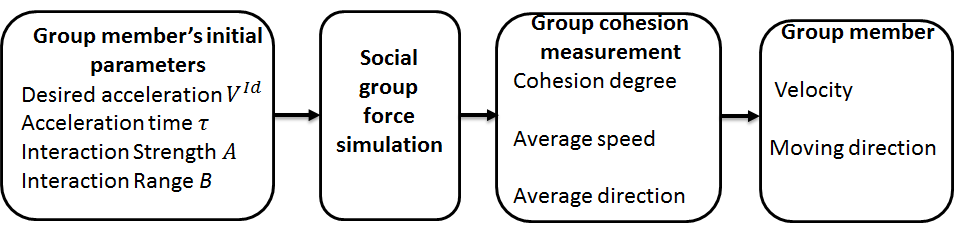
\includegraphics[width=0.05\columnwidth]{figs/parameter_impact.png}}
\end{center}
\caption{The methodology to understand the effect of group member's parameter on human group cohesiveness behaviour}
\label{fig:parameter_impact}
\end{figure}
Social-group force model is used in this study since its original social force model \cite{Helbing2000} sufficiently simulates human crowd’s self-organization phenomena in nature (e.g. lane formation, stop-and-go waves, bottleneck, turbulence phenomena) comparing to other crowd models \cite{Hoogendoorn2013}. Moreover, social force model was also co-invented by Vicsek, who invented the Standard Vicsek model, to design a particular model for simulating human movement.

Four group member’s parameters including desired acceleration $ \begin{math} \textit{V^{Id}} \end{math} $, acceleration time $ \tau $, interaction strength \textit{A} and interaction range \textit{B} are investigated since they are initial parameters of pedestrians in the model. 

Group cohesiveness is measured popularly by three factors including group cohesion degree, group average speed, and group average moving direction through major studies in the research field \cite{Vicsek1995} \cite{Czirok2000} \cite{Ballerini2008}. These factors are represented in equations (2.6), and (4.1-4.2). These factors are also particularly important for human group simulation because they support to represent occupied space for evacuation strategies and modelling collision avoidance of individual pedestrians when facing groups ahead.
\begin{equation}
\bar{v}_{group} = \frac{1}{N}\sum_{i=1}^{N}|v_{i}|
\end{equation}
\begin{equation}
\phi_{group} = \frac{1}{N}\sum_{i=1}^{N}|\vec{v}_{i}|
\end{equation}
where \textit{N} is group population size

This question is divided into two smaller questions which aim to explore parameter-cohesiveness relationship. In the first question, the following two aspects require careful consideration when designing experiments:
\begin{itemize}
	\item describe the range of possible model’s outputs of the three factors given by a set of inputs at the four model’s parameters where the parameters have uncertainty. Through providing the distributions of resulting outputs, it aims to support the predictive capacity of the model on human group cohesion behavior. 
	\item identify the key input parameters that contribute the most to the model’s outputs. By identifying the most influential parameters, it aims to improve the predictive capacity of the model by refining our estimates for those parameters.
\end{itemize}	
In the last question, understanding how different group cohesion factors affect individual group members is investigated.
\subsection{How do group member's parameters affect the model's outputs?}

This work relates to sensitivity analysis (SA) which aims to study how sensitive model's outputs are according to the variance of model’s inputs. The sensitivity analysis methodology have been applied widely in biological systems \cite{Marino2008}, \cite{Sumner2012},\cite{Hetherington2006}, water resource models \cite{Loucks2005}, traffic emission models \cite{Eriksson2007}, risk management models \cite{Hayes2011}, software engineering \cite{Williams2012},\cite{Wagner2007}, cellular signalling \cite{Hu2006}. This study investigates the effect of above four parameters by using Monte Carlos simulation (MCS). For a model with \textit{k} parameter inputs \begin{math} x =[x_{1}, x_{2}, x_{3},\ldots, x_{k}]\end{math}, MCS methodology involves the following steps \cite{Saltelli2000a}:
\begin{enumerate}
	\item Define distributions $ \begin{math} \textit{D_{1}},\textit{D_{2}},\textit{D_{3}},\ldots, \textit{D_{k}} \end{math} $ for the input \textit{x}
	\item Generate samples of size $ \begin{math} \textit{N}: \textit{x_{1}},\textit{x_{2}},\textit{x_{3}},\ldots, \textit{x_{N}} \end{math} $ from the defined distributions
	\item Run the model for each element in the input sample to obtain model's outputs $ y(x_{i}), \textit{i} \in [1,N] $
	\item Explore the mapping between uncertain inputs and the output uncertainty 	
\end{enumerate}
The output of MCS analysis is sensitive to the input distributions. The first step which characterises those distributions is the most important part in this technique as these distributions determine both the uncertainty y and the sensitivity of the elements of y to the elements of x (Saltelli, 2000b) (Helton, 2006). This step then considers two approaches: 1) define the simultaneously average distributions for four parameters 2) vary one parameter-at-a-time (OAT) which leaves fixed parameter values for remaining parameters by using their commonly values in Table~\ref{tab:model_params_values}.

In the second step, both random sampling and Latin hypercube sampling (LHS) are studied. LHS sampling procedure, which ensures the entire bins of each input are sampled, is also investigated since it has been shown to be more efficient than random sampling procedure \cite{Helton2006} and used in the analysis of a number of biological systems.  
 
In the third step, once the input samples have been generated for group members, social-group force model is simulated and the results of group cohesion measurement are stored over the time. Since this work requires a lot of computational resources and times; this step aims to perform simulation experiments on Monash clusters and apply their existing parametric frameworks such as Nimrod/G and Nimrod/E \cite{Abramson2011} to boost up collating the results from individual experiments.

The last step is to explore the effect of individual parameters on the model outputs at a certain time. This study uses following techniques including principal component, analysis, correlation analysis, regression analysis, and variance-based analysis, which are represented respectively as follows:
\begin{itemize}
	\item Principal Component analysis is the first effort to explore how model's parameters contribute to the model's outputs. This work is performed by: 1) extracting the first principal components (PCs) of input parameter combinations which give considerable model's output parameters. 2) mapping these PCs with model's outputs to give the first intuitive understanding of which parameters contribute to the variance of model's outputs.
		
	\item Correlation presents a measure of the strength of linear relationship between each model's parameter \textit{j} with model's outputs \textit{y}. It is measured by equations (4.3-4.4). In time-varying model, partial rank correlation coefficients are investigated on continuous time slices.
		\begin{equation}
			c(x_{j},y)=\frac{\sum_{i=1}^{N}(x_{ij}-\bar{x_{j}})(y_{i}-\bar{y})}{[\sum_{i=1}^{N}(x_{ij}-\bar{x}_{j})^{2}]^{1/2}[\sum_{i=1}^{N}(y_{i}-\bar{y})^{2}]^{1/2}}
		\end{equation}
		where
		\begin{equation}
			\bar{x}_{j}=\sum_{i=1}^{N}\frac{x_{ij}}{N}, \bar{y}=\sum_{i=1}^{N}\frac{y_{i}}{N}}
		\end{equation}
	\item Regression analysis provides a representation of the relationship between \textit{y} and multiple \textit{xj}'s as equations (4.4-4.5)
		\begin{equation}
			\hat{y} = b_{0} + \sum_{j=1}^{k}b_{j}x_{j}
		\end{equation}
		where the regression coefficients are determined such that the following sum is minimized
		\begin{equation}
			\sum_{i=1}^{N}(y_{i}-\hat{y}_{i})^{2} = \sum_{i=1}^{N}[y_{i}- (b_{0} + \sum_{j=1}^{k}b_{j}x_{ij})]^{2}
		\end{equation}
	\item Variance-based analysis deal when non-linear relationship of parameter j and model's output y. It partitions total output variance and identifies the amount of output's variation according to the uncertainty in the parameters.  Two main approaches of Fourier amplitude sensitivity test (FAST)\cite{Cukier1978} and its extension (eFAST)\cite{Saltelli1999}, which explore the parameters on frequency space, are investigated. Analysis of variance (ANOVA) method is also considered to examine the influence of each pair parameter on the model's outputs.
	\item Morris scanning design approach is used to rank the most influential parameter. It is based on OAT in which the investigating parameter is varied by small amount around its nominal point to identify the model behaviour in that region. Morris approach then repeats on different nominal points to measure the different outcomes. The approach is presented in Appendix A. The most influential parameters is then applied in simulation to visualize how group cohesion changes according the parameters.
	\item Another variance-based approach, Sobol method, is also considered to explore the impact of parameters on the model's outputs. Sobol method is based on the decomposition of the model's output into terms of increasing dimensionality and then compute the Sobol indices (the contribution) of each parameter to the variance of model output. The method is presented in Appendix~\ref{app:1} as well. 
\end{itemize}	

\subsection{How does group cohesion behavior affect group member’s velocity and direction over the time?}
This question investigates the effect of group cohesion on group members according to their initial parameter settings. It aims to understand how group members need to limit their individuality in order to align their behavior with their group mates. Two prototypes including individuals moving in group compared with when those same individuals behave individually are compared on the variance of each individual’s speed and direction when tested on its own. It is called as individual-level conformity.

This work has been approached in the research of schooling fishes \cite{Herbert2012} through linear mixed-effects model to assess the effect of context (parameters of other group members on parameters of current considering group member). This work is then applied to consider for each group member to generalize the effect. Other information such as panic level (the variance of actual speed over desired speed) of individuals is also investigated.

\section{How does group cohesion behavior affect flow rates?}
This question aims to investigate the impact of group cohesion behavior on flow rates in various simulation scenarios of corridors and evacuations comparing to individual behavior. This work is based on parameter selections which produce different group cohesion behaviour in Question 1.1. Designing simulations aims to scrutinize how group cohesion behavior can help individual group members avoid effectively obstacles and how out-group pedestrians are affected in route choice when facing groups. 
\begin{itemize}
	\item Scenario 1: Move with group comparing to move individually to avoid obstacles.
	\item Scenario 2: Group members interact with out-group individuals in corridor and evacuation simulation environments.
\end{itemize}
In general, factors influence flow rates are caused by low-velocity of individuals, route choice when facing dynamic obstacles, and the occurrence of self-organization phenomena (bottleneck, lane formation, freeze-by heating). Thus, trajectories of individual members and forces affecting them are tracked to investigate these reasons in each scenario. In the last scenario, different layouts including multiple corridors leading to a unique evacuation door and placements of pedestrians are also considered thoroughly. Trajectories of out-group members also collected to investigate the effect of group members of these pedestrians. 

The change of flow rates is also investigated when varying group member’s parameters based on parameter ranking to determine areas in which flow rates change smoothly or disordered. 

\section{What is the impact of group member's parameters on group cohesion behaviour and flow rate measurement when group member are heterogeneous in parameter distributions?}
Since previous models consider group members and out-group pedestrians as homogeneous particles through using the same parameter values, a recent calibration study \cite{Daamen2012} found that different pedestrians in age (children $ \leq 14 $ years old, adults, elders $ \geq 65 $ years old) have different distributions in individual parameters to those of others in evacuation scenarios. These scenarios were setup by recording and tracking pedestrians escaping a narrow door under emergency and light sounds.
Thus, the initial exploratory step in this question is to find the difference between setting different parameter distributions and setting an average distribution via flow rate measurement. This analysis is presented in Appendix~\ref{app:2}. The average distribution is considered among normal average distribution, normal distribution with constraints, uniform distribution, and uniform distribution with constraints. This work is to help us fundamentally understand the importance of setting different parameter distributions for heterogeneous pedestrians in simulation scenarios including moving along corridors or escaping a bottleneck. 
The next step will perform similarly as Questions 1 and 2 on each group type (purely unique group member type, different group member types). OAT approach is applied to measure the effect of each parameter. At each considering parameter, the values of group members at that parameter are sampled repeatedly from the parameter’s distribution. These values are kept unchanged when investigating other parameters.

\chapter{Research project's contribution}
\let\cleardoublepage\clearpage
This study will enable modellers understand following impacts of member's parameter settings on group cohesion behavior.
\begin{itemize}
	\item which parameter contribute most to the variance of group cohesion behavior
	\item how group cohesion affect individual group members
	\item the impact of group cohesion behaviour on flow rate measurement which has not been explored by previous human crowd models
\end{itemize}
Understanding the role and interaction effect of parameters on the model’s outputs helps to improve the performance of real-time prediction systems based on these models by: 
\begin{itemize}
	\item Refining and concentrating on the most influential parameters for real-time extraction systems to enhance these studies \cite{Moore2011} which applied the social-force model for real-time abnormal-behavior detection system.
	\item Predicting empty and occupied space for evacuation plan and crowd's possible behavior from known parameter distributions of pedestrian types in crowd before deteriorative situations can occur.
\end{itemize}

\chapter{Research progress}
\let\cleardoublepage\clearpage
This section presents current working progress on the implementation of social-group force model and preliminary analysis of group member’s parameters in sections 6.1 and 6.2. The research timeline in the last section 6.3 is to represent continuous phases to resolve the next questions in the rest period of this PhD study.
\section{The implementation of social group force model}
\subsection{Simulation Techniques}
Our simulation is developed with following configuration. Social group force model is implemented on C library for performance purpose. Below packages are used to initialize simulation and obtains group cohesion degree, average speed and velocity direction over the time.
\begin{itemize}
	\item Python version 3.4.1
	\item Numpy library version 1.8.1 is used to generate Gauss distribution for pedestrian’s parameter values.
	\item Matplotlib library version 1.3.1 is used to plot our measuring results.
	\item Pygame engine version 1.9 to visualize obstacles and update pedestrian’s position with a frame rate of 100 fps.
\end{itemize}
The simulation allows pedestrians start at a specific area and move to reach the predefined target. We use Euler’s method to update new velocity and position of each pedestrian as in equations (6.1-6.2).
\begin{equation}
			p(t + \Delta t)=\frac{1}{2}\alpha\Delta t^{2} + V(t)\Delta t + p(t)
\end{equation}
\begin{equation}
			V(t + \Delta t)=\alpha\Delta t + V(t) 
\end{equation}
where \textit{p} is the position, \textit{V} is the velocity, a is the total combinatorial acceleration given by the model in equation (2.8) or total force given by force model in equation (7). \begin{math} \textit{\Delta t} \end {math}is the time step and set \begin{math} \textit{0.01} \end{math} second to perform real-time crowd modelling.
Cartesian coordinator system is applied on Pygame’s screen with a pixel factor to simulate the pixel number per meter. \begin{math} \textit{O(0,0)} \end{math} root coordinator is aligned at the centre of simulation screen.

\subsection{Parameter initialization and social-group force model output's processing}
In our simulation, a group of \textit{N} = 4 group members is generated. This group size is considered as more frequent than other larger group sizes \cite{Moussaid2010} since larger groups are also automatically split into subgroups of 3-4 members. Group members are predefined in our simulation environment rather than considering neighbors as group members.
\begin{figure}[ht]
\begin{center}
\resizebox{130mm}{!}{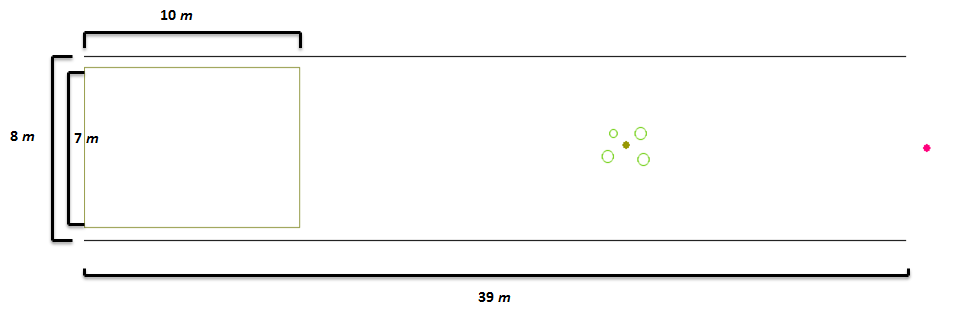
\includegraphics[width=0.05\columnwidth]{figs/scenario_uniflow.png}}
\end{center}
\caption{Group cohesion simulation based on social group force model in unidirectional flow}
\label{fig:scenario_uniflow}
\end{figure}
Group members are represented as green circles. Initial placements for these members are randomly in the designated yellow area. Radius of group members are generated from normal distribution \begin{math}(\mu_{radii}=0.3\end{math} and \begin{math} \sigma_{radii}=0.05) \end{math} as suggested by previous study \cite{Helbing2000}. 
In this study, possible ranges of group member’s parameters are represented as below table. They are collected from the literature reviews of Helbing's and colleague's studies.
\begin{table}[H]
\caption{Social-group force model’s parameter ranges}
\begin{center}
\begin{tabular}{|l|l|l|} \hline
\textbf{Parameter} & \textbf{Range[min-max]} & \textbf{Step to vary} \\ \hline
\begin{math}\textit{V_{p}^{Id}(m/s)}\end{math}&[1.0-3.0]&0.2 \\ \hline
\begin{math} \textit{\tau(s)} \end{math}&[0.2-2.0]&0.2 \\ \hline	
\textit{A}(m/s^{2})&[1.0-4.0] &0.2\\ \hline
\textit{B}(m)&[0.2-2.0]&0.2\\ \hline																										
\end{tabular}
\end{center}
\label{tab:model_params_ranges}
\end{table}
Totally, there contains more than 17000 combinations. Parameter values at each combination are applied the same for group members.
Due to the highly computational resources, Monash Cluster Campus (MCC) has been used to deploy the simulation and obtain group information outputs including cohesion degree, average speed, and average velocity direction over the time. The system ran for more than five days to complete above parameter combination number.

Each parameter combination is simulated \textit{n}= 15 times in which each running time contains different placements and radii for group members. These placements and radii are kept for all above parameter combinations in order to purely investigate the impact of member's parameters on group cohesion outputs. Each simulation time is limited at 100 second period or the simulation can finish as all group members has reached the defined target.

The first ten second period and the last five second period in the time series of each group information output are eliminated in order to make sure the group pattern is emerged regardless initial placements of group members or some of group members reached the target. A running time's outputs is then normalized and averaged as a scalar value from this time series. The model's outputs are then averaged by these \textit{n} running times.

\section{Group cohesion measurement based on group member's parameters}
Due to the large sample size (more than 17000) of group information output, \texit{k} highest and lowest values at each bin with the length \textit{0.2} is extracted for understanding how group information vary according to possible combinations of four considering parameters. Moreover, due to the high dimensionality of these input parameters \begin{math} {\textit{V_{p}^{Id},\textit{\tau(s)},\textit{A},\textit{B}}\end{math}, PCA is applied to transform them into a new smaller dimensional space.
\subsection{The variance of group cohesion degree}
Parameter combinations giving minimum and maximum group cohesion degree values in bins are used to extract the first principle components \textit{(PCs)}. Figure ~\ref{fig:group_cohesion_pca_weight} represents how much variance of parameter inputs can be attributed to each of PCs. Totally, the first two PCs can illustrate more than 60 percentage of variance in the parameter combinations.
\begin{figure}[H]
\begin{center}
{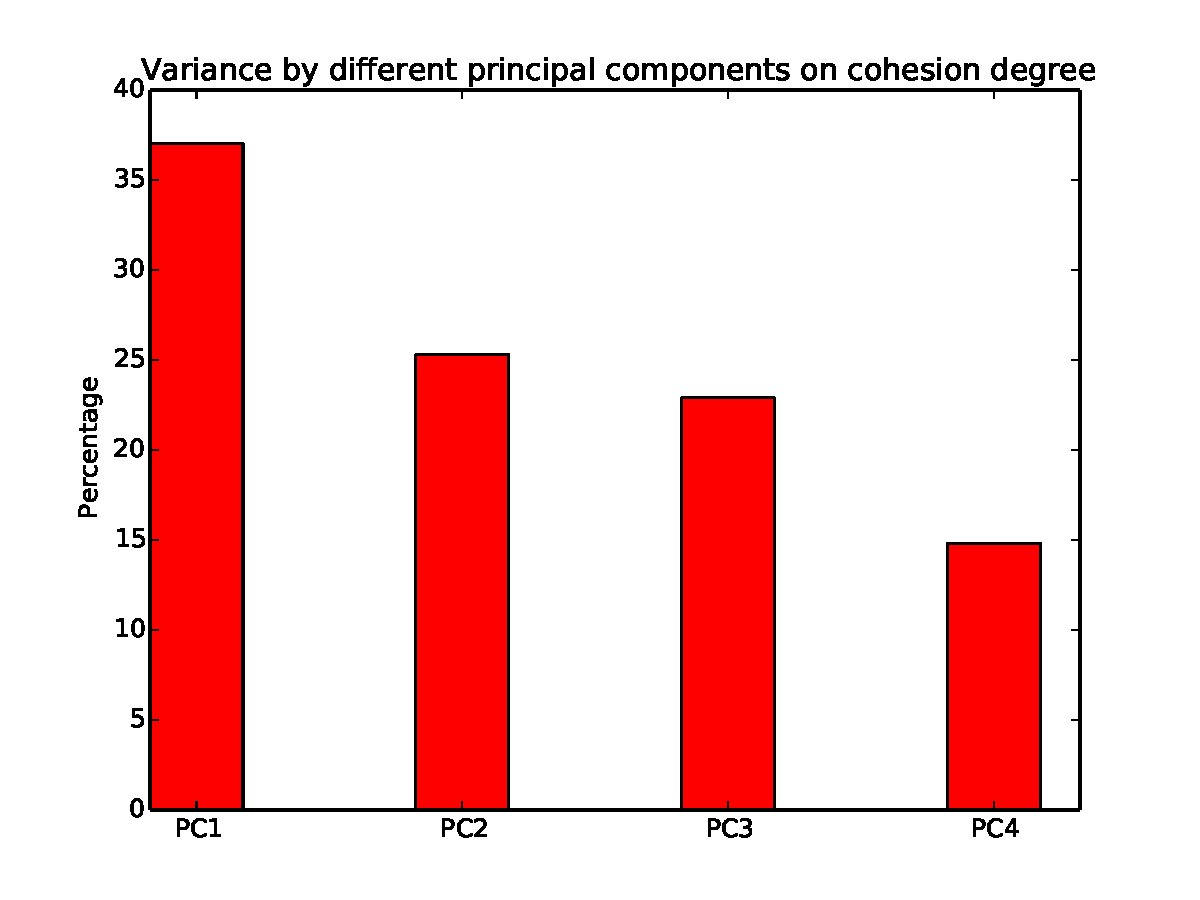
\includegraphics[width=8cm,height=8cm]{figs/pc_c_d.pdf}}
\end{center}
\caption{Contribution of principal components of parameters on group cohesion degree}
\label{fig:group_cohesion_pca_weight}
\end{figure}
Parameter combinations are then transformed into a new space identified by the first two PCs. Figure ~\ref{fig:pca_corr_group_cohesion} presents the proportion of variances of four parameters explained by each components. The first component correlates the most with \textit{Interaction Strength} and \textit{Interaction Range}. The second PC shows the highest correlation value with \textit{Desired Velocity} comparing to other parameters.
\begin{figure}[H]
\begin{center}
{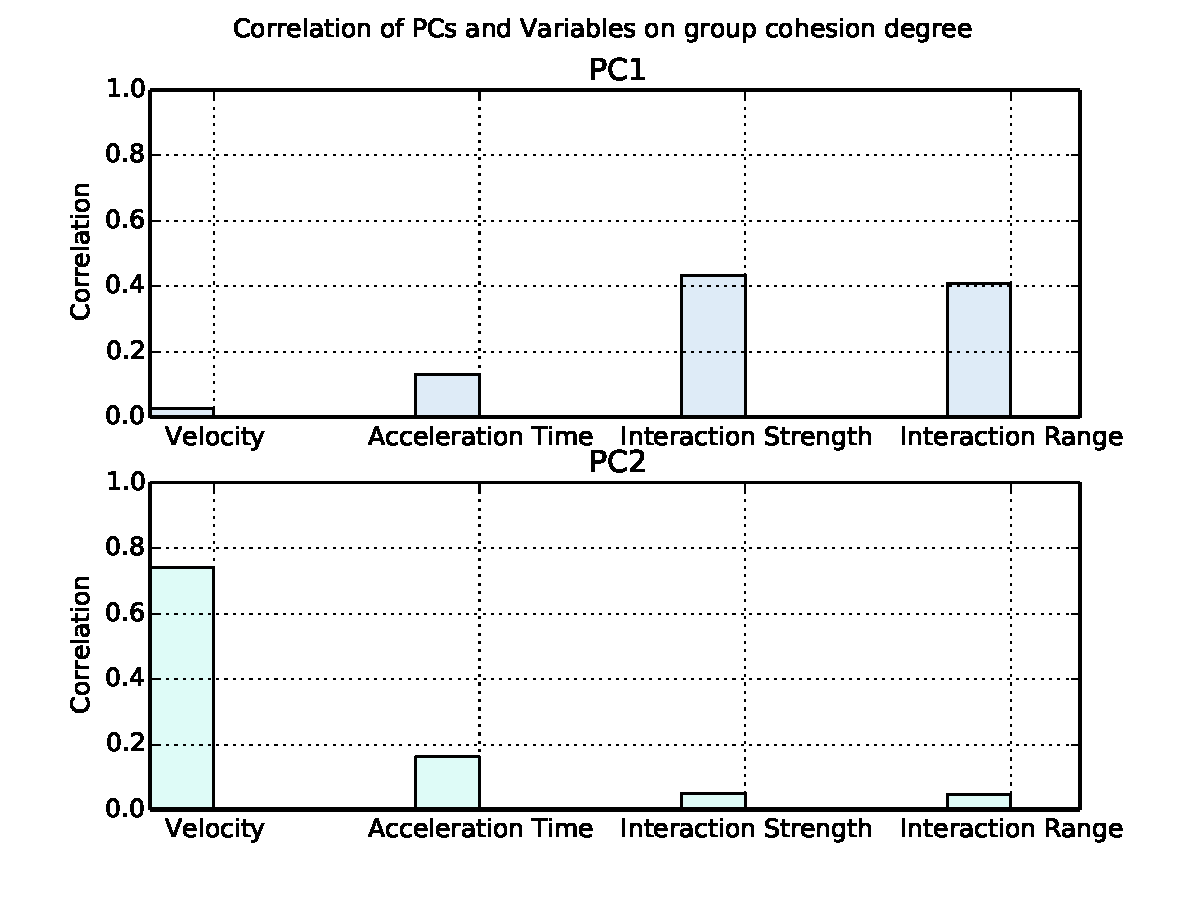
\includegraphics[width=8cm,height=8cm]{figs/pca_corr_group_cohesion.pdf}}
\end{center}
\caption{Correlation between the first two PCs and model's input parameters on group cohesion}
\label{fig:pca_corr_group_cohesion}
\end{figure}
Figure ~\ref{fig:pca_lanscape_group_cohesion} presents the relation between the first two PCs and group cohesion degree. Particular red dots give the lowest values of group cohesion degree; it is expected low degree of group cohesion is contributed by low values of parameters \textit{Interaction Strength} and \textit{Interaction Range}. On the PC2 axis, group cohesion almost vary at high values represented by blue dots. Since this PC correlates the most with parameter \texit{Desired Velocity}; thus it implies that high degree of group cohesion contains the contribution of group member's velocity.
\begin{figure}[H]
\begin{center}
{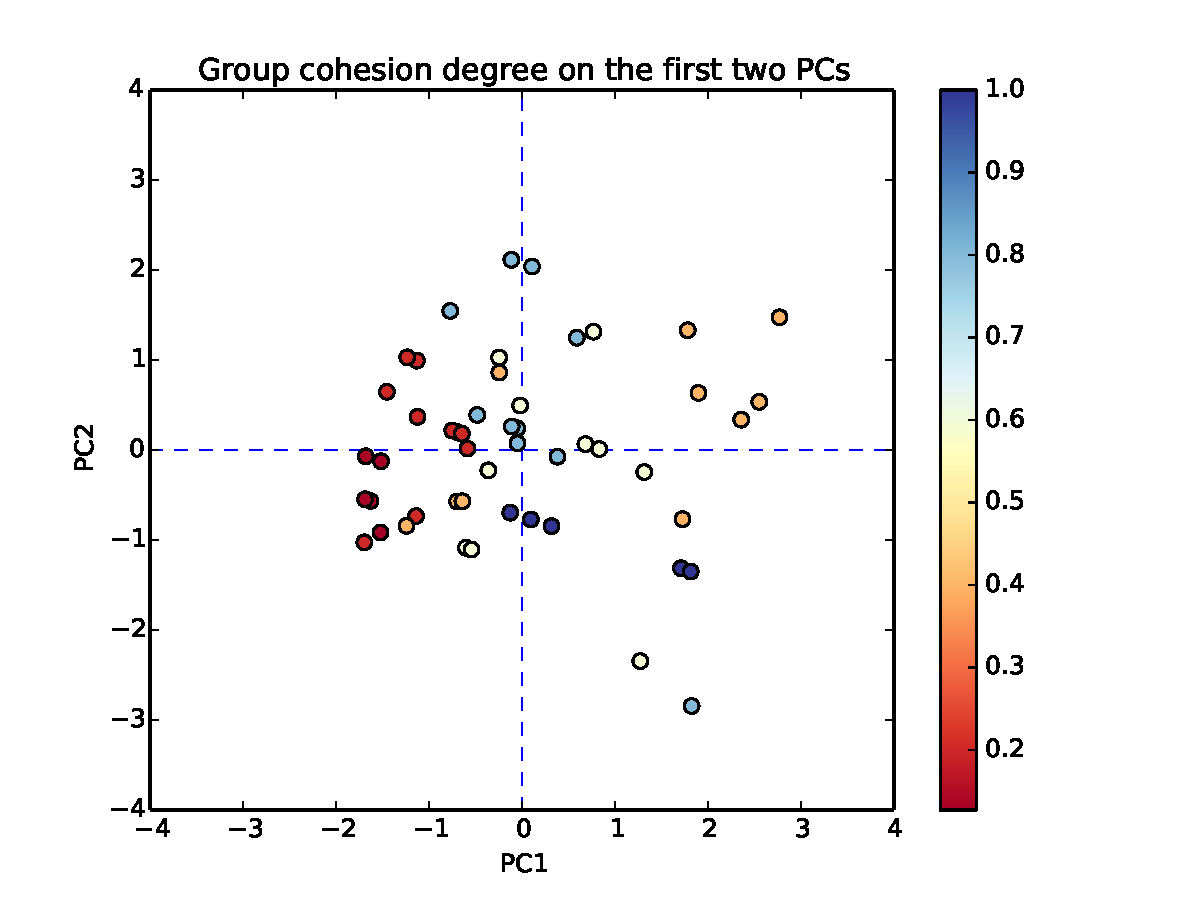
\includegraphics[width=7cm,height=7cm]{figs/pca_lanscape_group_cohesion.pdf}}
\end{center}
\caption{Relation between the first two PCs and group cohesion degree}
\label{fig:pca_lanscape_group_cohesion}
\end{figure}

\subsection{The variance of group average speed}
Figure ~\ref{fig:pca_corr_group_speed} presents the proportion of variance of four parameters explained by the first two PCs which give minimum and maximum values of group's average speed. Parameter \textit{Interaction Strength} and \textit{Desired Velocity} have strong correlation with the first and second components respectively. The contribution of these PCs on the variance of group member's parameters is presented in Figure ~\ref{fig:pc_a_s.pdf}. 
\begin{figure}[H]
\begin{center}
{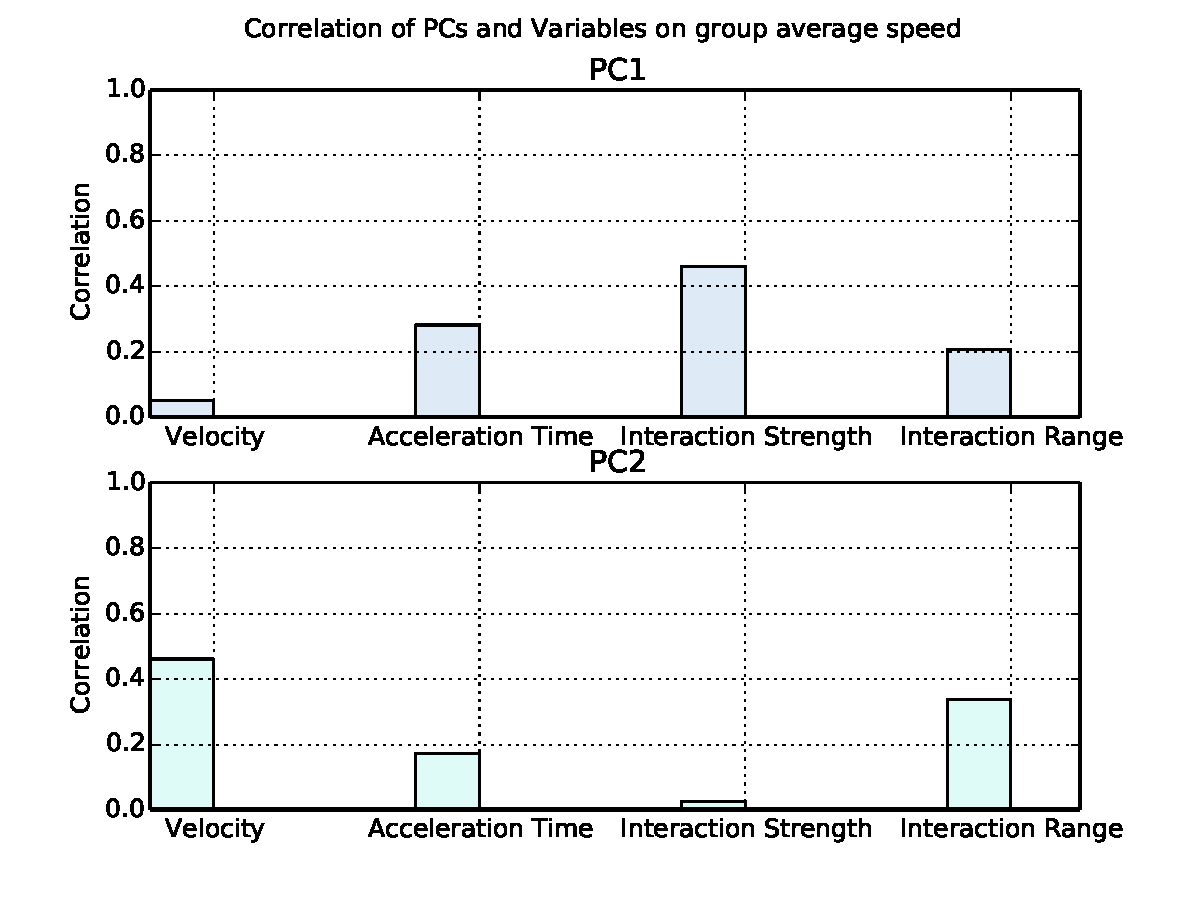
\includegraphics[width=7cm,height=7cm]{figs/pca_corr_group_speed.pdf}}
\end{center}
\caption{Correlation between the first two PCs and model's input parameters on group speed}
\label{fig:pca_corr_group_speed}
\end{figure}
\begin{figure}[H]
\begin{center}
{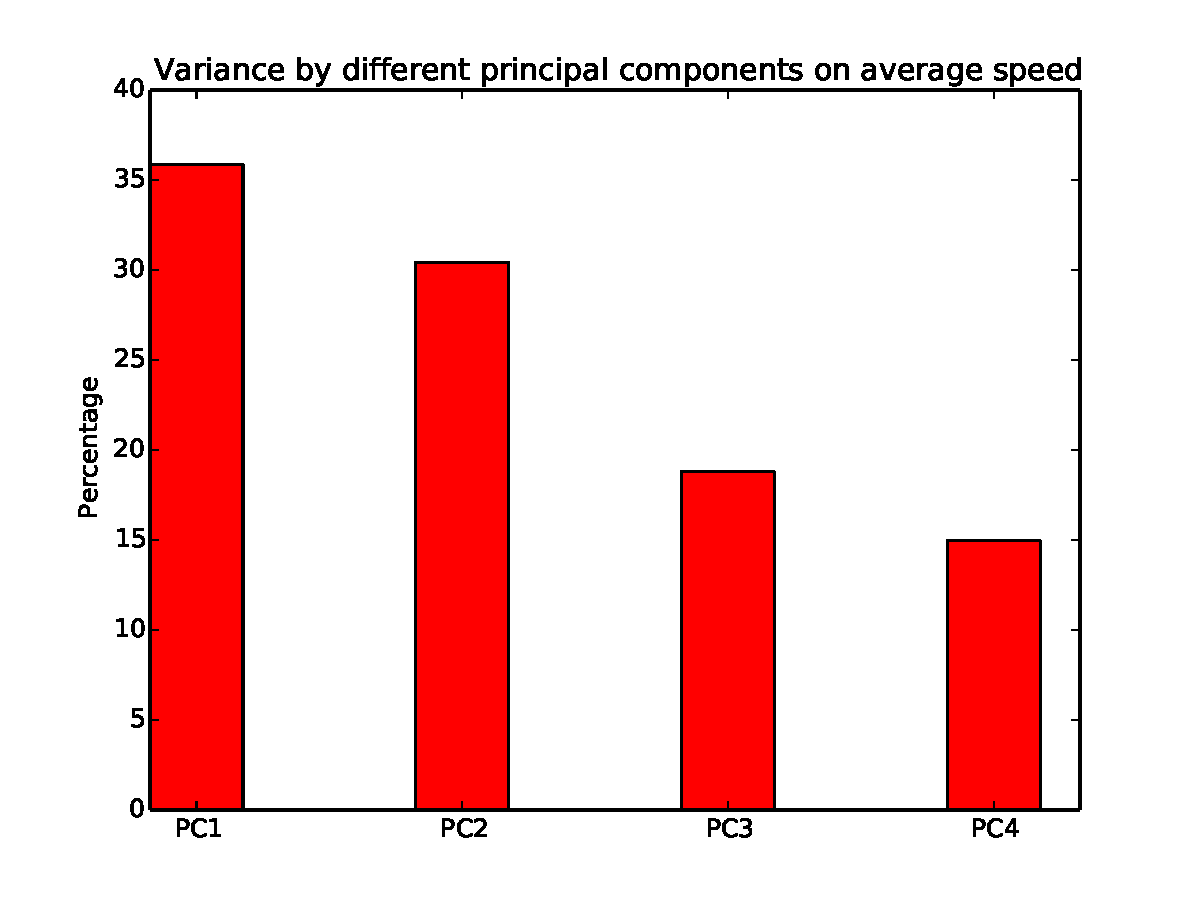
\includegraphics[width=7cm,height=7cm]{figs/pc_a_s.pdf}}
\end{center}
\caption{Contribution of the first two PCs of parameters on group average speed}
\label{fig:pc_a_s.pdf}
\end{figure}
The relation of the first two PCs and group average speed is presented in Figure ~\ref{fig:pca_lanscape_group_speed}. The variance of group average speed is separated clearly on PC1. Red dots present low value of group's average speed. Blue dots at farther points from mean value \textit{0} show high values of \textit{Interaction Strength}. Parameter \texit{Desired Velocity} also has a less contribution on group average speed since the variance of group's average speed is small while the variance of PC's values is higher. 
\begin{figure}[H]
\begin{center}
{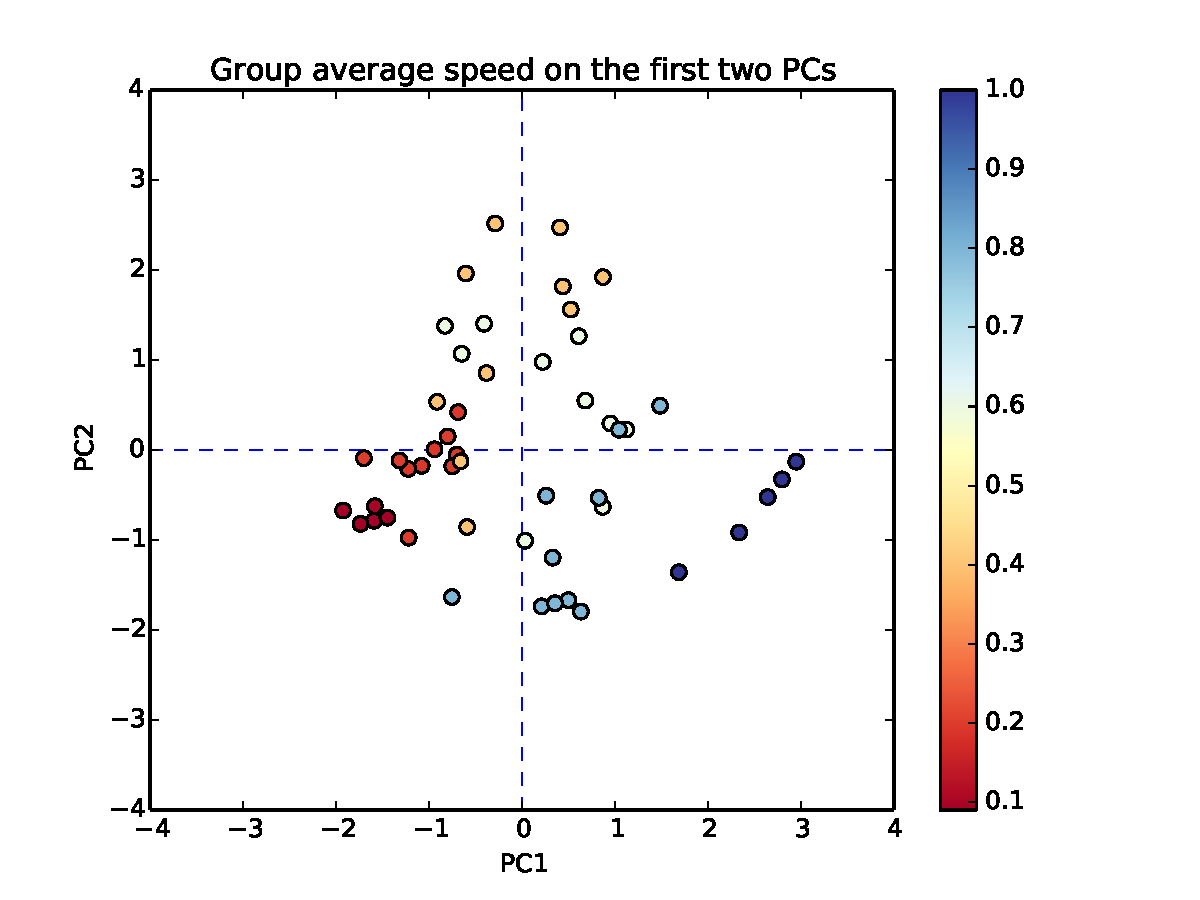
\includegraphics[width=7cm,height=7cm]{figs/pca_lanscape_group_speed.pdf}}
\end{center}
\caption{Relation between the first two PCs and group average speed}
\label{fig:pca_lanscape_group_speed}
\end{figure}

\subsection{The variance of group average velocity direction}
This section presents the contribution of group member's parameters to the variance of group velocity direction. Figure ~\ref{fig:pc_a_d} describes the weight of the first two principal of four-dimensional parameter combinations giving minimum and maximum values of group velocity direction on same-size bins. Totally, the first two PCs can generate more than 70\% the variance of group velocity direction.    
\begin{figure}[H]
\begin{center}
{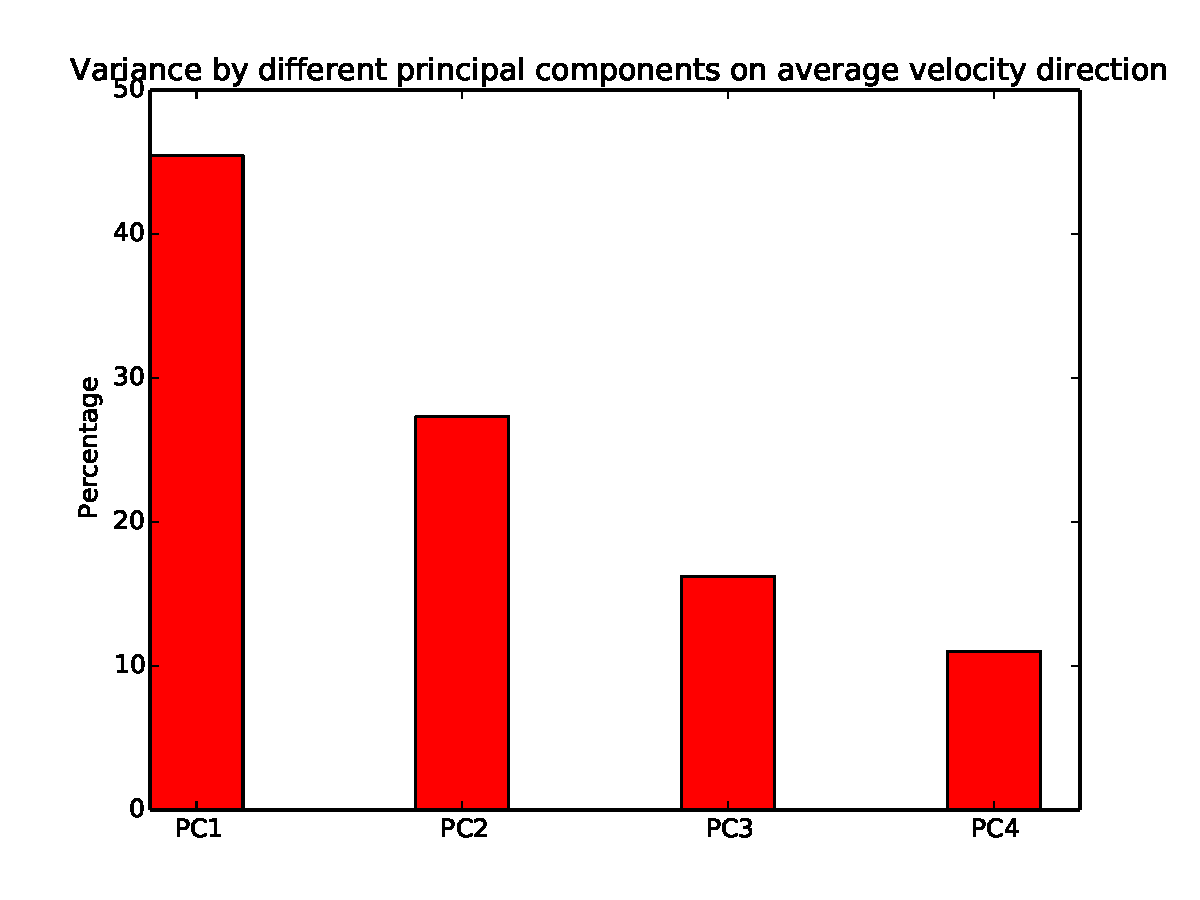
\includegraphics[width=7cm,height=7cm]{figs/pc_a_d.pdf}}
\end{center}
\caption{Contribution of principal components of parameters on group velocity direction}
\label{fig:pc_a_d}
\end{figure}
The correlation between these PCs and group member's parameters is shown in Figure ~\ref{fig:pca_corr_group_direction}. The first PC correlates with \textit{Interaction Strength} and \textit{Interaction Range}. The second PC is proportional with the parameter \textit{Desired Velocity}.
\begin{figure}[H]
\begin{center}
{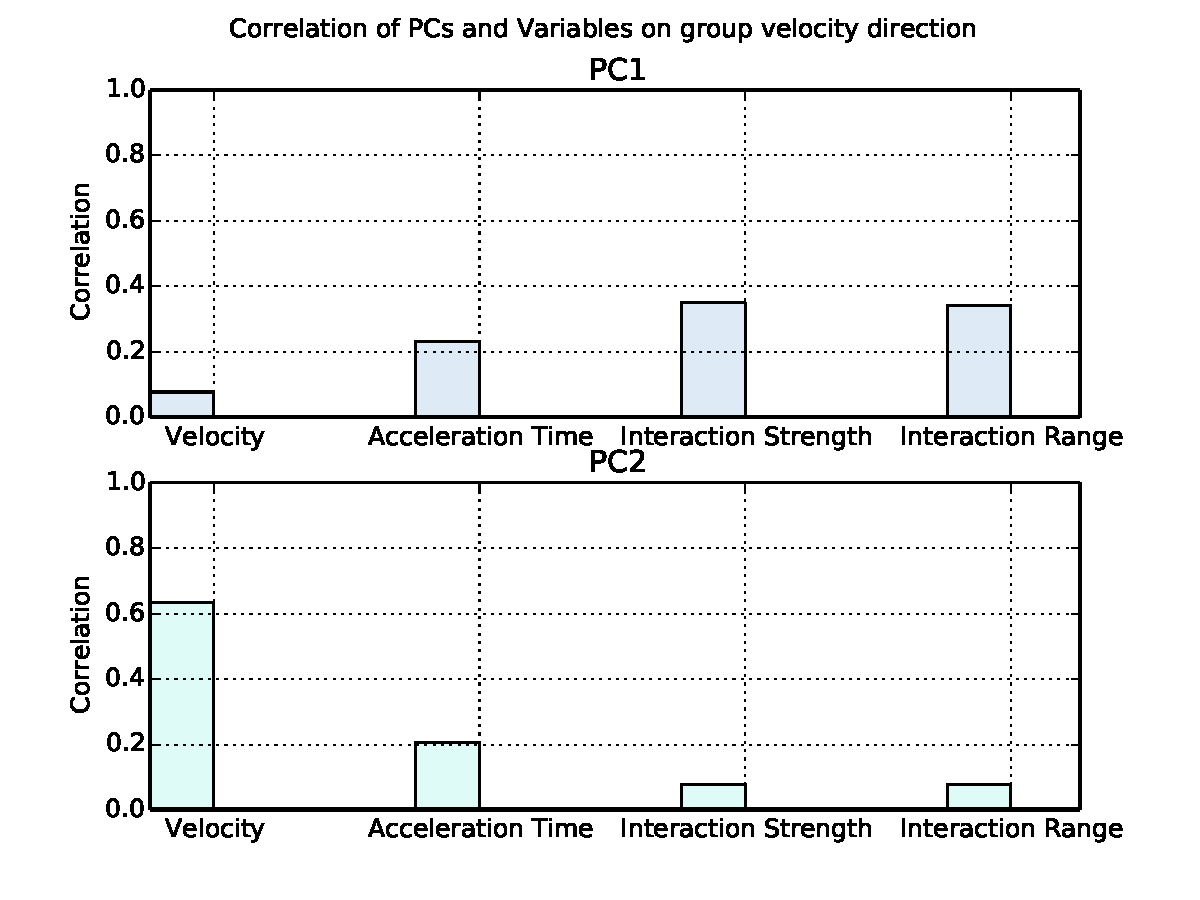
\includegraphics[width=7cm,height=7cm]{figs/pca_corr_group_direction.pdf}}
\end{center}
\caption{Correlation between the first two PCs and model's input parameters on group velocity direction}
\label{fig:pca_corr_group_direction}
\end{figure}
\begin{figure}[H]
\begin{center}
{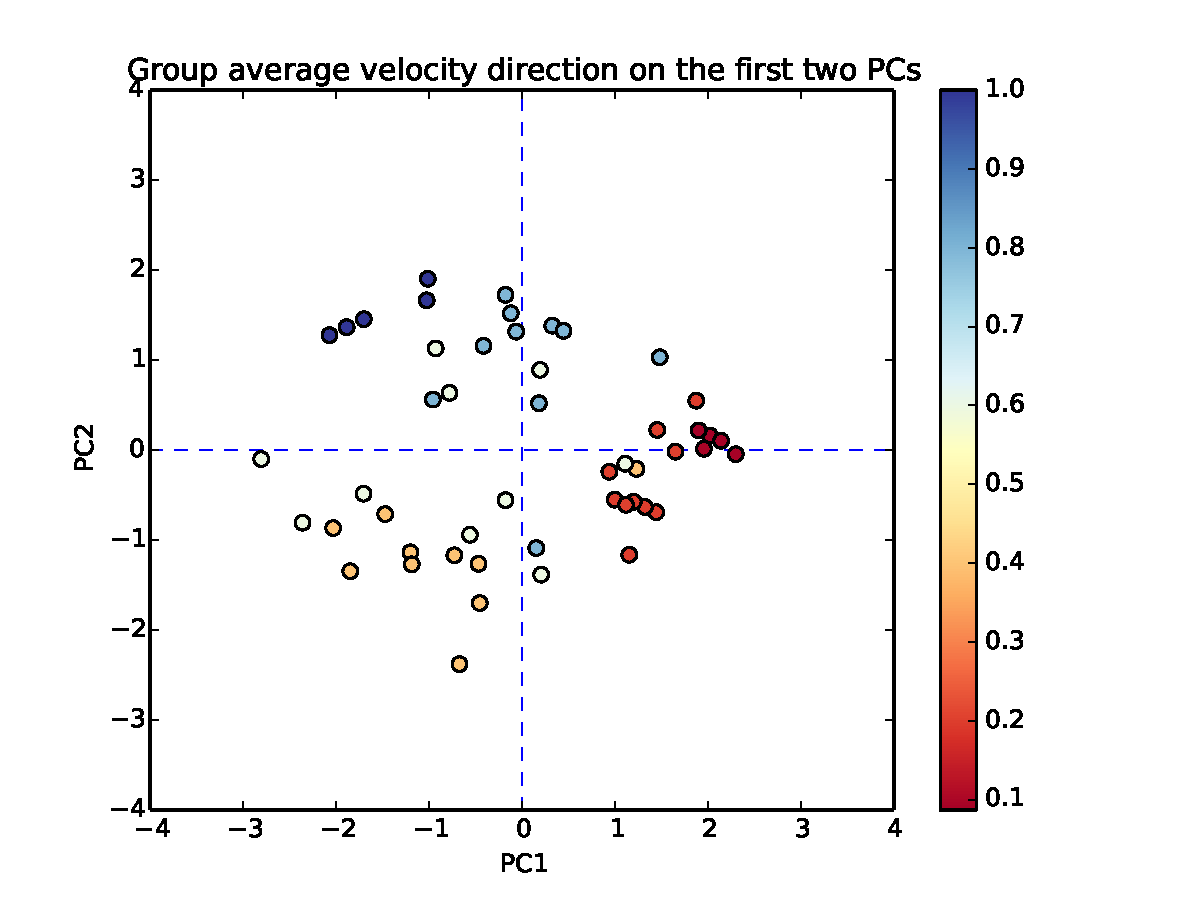
\includegraphics[width=7cm,height=7cm]{figs/pca_lanscape_group_direction.pdf}}
\end{center}
\caption{Relation between the first two PCs and group average direction}
\label{fig:pca_lanscape_group_direction}
\end{figure}

Figure ~\ref{fig:pca_lanscape_group_direction} shows that high value of group's average velocity direction is contributed by low value of \textit{Interaction Strength} and high value of \texit{Desired Velocity}. However, minimum values of group's direction represented by red dots are influenced more by \textit{Interaction Strength}.  

\subsection{Summary}
From the above experiment, we can see that the parameters \textit{Interaction Strength}, \textit{Interaction Range}, and \textit{Desired Velocity} almost contribute mainly to the minimum and maximum values of the model's outputs. Specifically, minimum value of group cohesion degree is influenced by parameters of repulsive force (\textit{Interaction Strength}, \textit{Interaction Range}). In the observation of group's average speed and direction, \textit{Interaction Strength} contributes to both of minimum and maximum values. However, there is still remain more works should be done to investigate and verify. Above analysis also remains several limitations:
\begin{itemize}
	\item PCA only deals with linear interaction by decomposing original data to the sum of principal components; thus, the first PCs still can not illustrate fully the variance of input parameters
	\item The model's outputs are not normal distribution 
\end{itemize}
Therefore, below tasks are undertaken to help us explore more deeply on the role of group member's parameters to resolve the proposed research questions.
\begin{itemize}
	\item Applying analysis of variance to measure the effect of each pairs of two parameters
	\item Applying Sobol and Morris algorithms to deal with sensitivity analysis
\endd{itemize} 

\section{Research Timeline}

The prospective sub-tasks are planned as Figure~\ref{fig:research_timeline} to push this PhD study move forward and achieve expected publications through the proposed research questions on time.
\begin{figure}[H]
\begin{center}
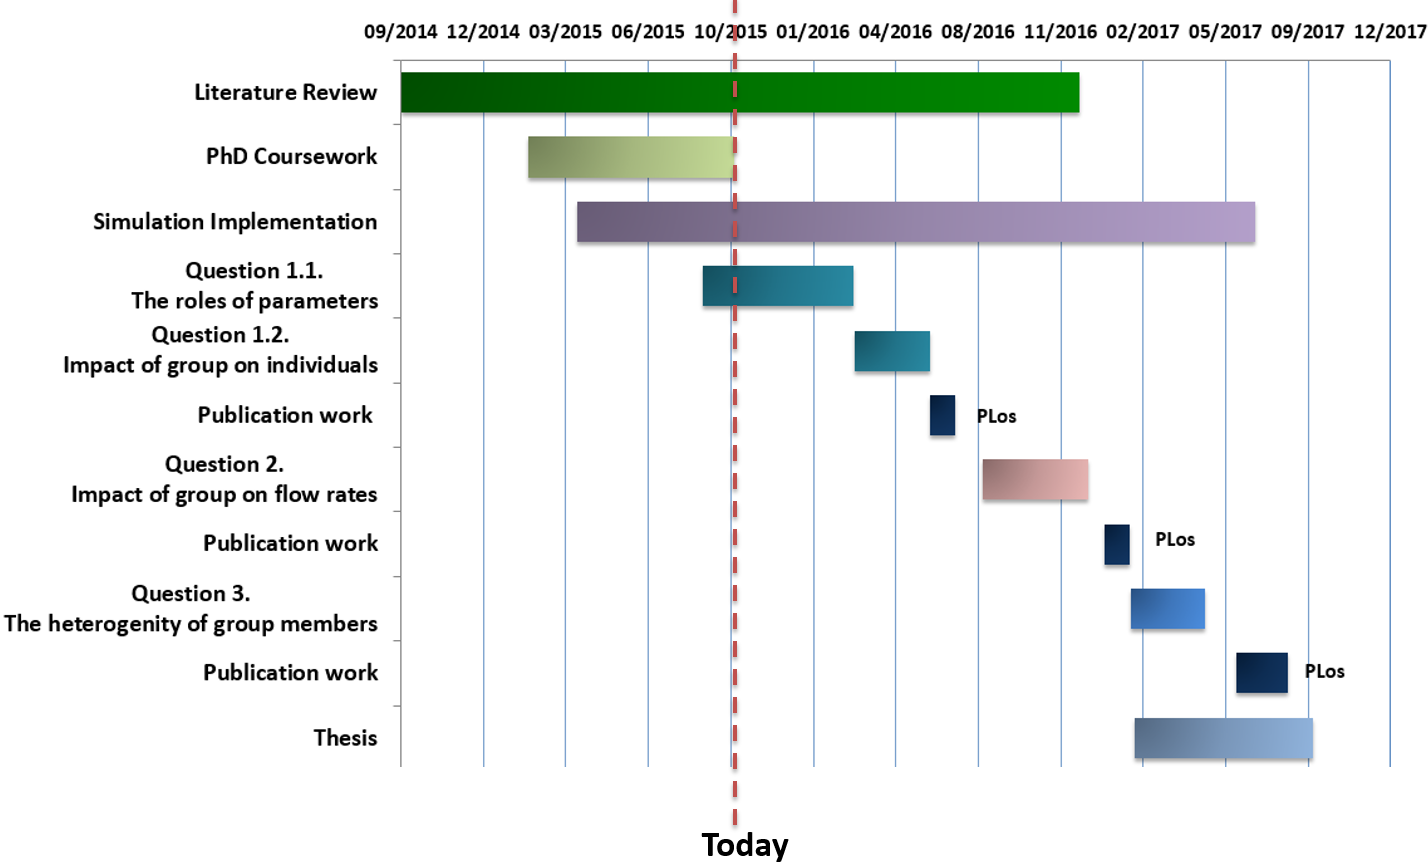
\includegraphics[width=0.8\columnwidth]{figs/research_timeline.png}
\end{center}
\caption{Research Timeline}
\label{fig:research_timeline}
\end{figure}

\chapter{Coursework and professional development}
\let\cleardoublepage\clearpage
As required from our faculty, I completed the course FIT 5143 in the first semester 2015 and the course FIT 6021 in the second semester 2015. I also completed 116 research training hours out of 121 compulsory research training hours as in Table~\ref{tab:research_training}.
\begin{table}[H]
\caption{List of professional development undertaken}
\begin{center}
\begin{tabular}{|l|l|} \hline
\textbf{Activity} & \textbf{Hours counted towards coursework goal}\\ \hline
Faculty Induction&4 \\ \hline
Research Integrity&12 \\ \hline
FIT 5143&Course	Completed \\ \hline
FIT 6021&Course Completed \\ \hline
FIT 4012&15 \\ \hline
Monash Seminar/workshop attendance&22 \\ \hline
Monash Bootcamp Commercialisation 2015&15 \\ \hline																									
\end{tabular}
\end{center}
\label{tab:research_training}
\end{table}

\appendix % all \chapter{..} commands after this will generate appendices
\chapter{Sensitivity Analysis Methods}
\label{app:1}
Sensitivity analysis (SA) describes how sensitive the model's output are to the variation of individual input parameters. It helps to determine which parameter lead the majority of the variation in the output. Sensitivity analysis has been used widely in research fields of biological systems to enhance the understanding of complex computational models, seeking inputs which have substantial effect on particular outputs, constructing an emulator/reduced model. 
Ranking the most sensitive parameters and their interaction effect with other parameters are often performed by Morris and Sobol approaches.
\begin{itemize}
	\item Morris scanning approach: consider \begin{math} \textit{y(P)} \end{math} is an output of the model at parameter point \textit{P} where \textit{P} is vector of parameter values at \begin{math}(\textit{p_{1}}, \textit{p_{2}}, \textit{p_{3}},\ldots, \textit{p_{k}}) \end{math}. The Morris method defines the elementary effect of \begin{math} \textit{i^{th}} \end{math}parameter at \textit{P} as:
	\begin{equation}
			d_{i}=\frac{y(\textit{p_{1}},\ldots, \textit{p_{i-1}},\textit{p_{i} + \Delta},\textit{p_{i+1}, \ldots,\textit{p_{k}}})-y(\textit{P})}{\Delta}\frac{\sigma_{p_{i}}}{\sigma_{y}}
	\end{equation}
	where \begin{math}\Delta \end{math} is selected such that \begin{math} \textit{P + \Delta} \end{math} is still in the set of allowable values for parameter \textit{k}
	\item Sobol approach: Given a model of the form \begin{math} \textit{y(t)=f(u,P,t)} \end{math} where model's output \begin{math} \textit{y(t)} \end{math} is a set of curves describing the variation in the model output over time, \textit{u} is external model input, and a set of \textit{k} parameters represents model's considerable parameters \begin{math} (P =(\textit{p_{1}}, \textit{p_{2}}, \textit{p_{3}},\ldots, \textit{p_{k}})) \end{math}. The function \textit{f} can be represented as:
	\begin{equation}
	f(\textit{p_{1}}, \textit{p_{2}}, \textit{p_{3}},\ldots, \textit{p_{k}}) = f_{0} + \sum_{j=1}^{k}f_{i}(p_{i}) + \sum_{1 \leq i  \leq j  \leq k}f_{ij}(p_{i},p_{j}) \\ + \ldots + f_{1,2,\ldots,k}(p_{1},p_{k})
	\end{equation}
\end{itemize}

\chapter{The impact of setting different parameter distributions for pedestrian types}
This appendix presents current working progress to examine the difference in flow rates when setting different parameter distributions and averaging out the same parameter distribution for pedestrian types. This appendix only considers pedestrians moving individually to reach a target point without group force.
\section{Parameter distribution initialization for pedestrian types}
According to the calibration study \cite{Daamen2012}, parameters including desired acceleration \begin{math} \textit{V^{Id}} \end{math}, acceleration time \begin{math}\tau \end{math}, interaction strength \textit{A}, and interaction range \textit{B}  in Table~\ref{tab:model_params_values} are different between pedestrian types of children (to age 14), adults, and elders (age 65 and older) in emergency situation. Elderly people are more aggressively to walk with their desired speed than children do. For the interaction strength parameter, the strength of children is strongest comparing to those values between adults and elderly in a population with a large heterogeneity. In the last parameter, children have the lowest value; it implies that the interaction force affecting children can be easier changed by distance than it does on elders and adults. However, the study also mentioned that the standard deviation of each pedestrian type's parameters was not stable. It was due to the fact that the study was calibrated in various simulated scenarios which involves different percentages of these pedestrian types. Thus, in this study we consider:
\begin{equation}
 \sigma_{c_{children}}=k\mu_{c_{children}}, \sigma_{c_{adult}}=k\mu_{c_{adult}}, \sigma_{c_{elder}}=k\mu_{c_{elder}}
\end{equation}
where:
\begin{itemize} 
	\item \textit{c} is control parameter in  \begin{math} S=\{\textit{V^{Id}},\tau,\textit{A},\textit{B}\}\end{math}
	\item \textit{k} is base parameter, \textit{k} = 0.1
\end{itemize}

Table~\ref{tab:model_params_dist} represents parameter distributions for pedestrian types on this approaches based on common values taken from Table ~\ref{tab:model_params_values} of the original social force model.
\begin{table}[H]
\caption{Parameter distributions for three pedestrian types}
\begin{center}
\begin{tabular}{|l|l|l||l|l|l|l|} \hline
\multirow{3}{*}{Social Force Parameters} & \multicolumn{6}{c|}{Pedestrian type's parameters} \\ 
														  \cline{2-7} &
															\multicolumn{2}{c|}{Children} & \multicolumn{2}{c|}{Adult} & \multicolumn{2}{c|}{Elder} \\ 
															\cline{2-7} & \begin{math}\mu\end{math} & \begin{math}\sigma\end{math} &
															\begin{math}\mu\end{math} & \begin{math}\sigma\end{math} &
															\begin{math}\mu\end{math} & \begin{math}\sigma\end{math} \\ \hline
\begin{math}V^{Id}(m/s)\end{math}&1.7&0.17&1.3&0.13&0.9&0.09\\ \hline
\begin{math}\tau(m/s)\end{math}&1.3&0.13&1.0&0.1&0.5&0.05 \\ \hline
\textit{A}(m/s^{2})&4.0&0.4&3.0&0.3&2.0&0.2\\ \hline
\textit{B}(m)&0.13&0.013&0.3&0.03&0.2&0.02\\ \hline	 																										
\end{tabular}
\end{center}
\label{tab:model_params_dist}
\end{table}
Mean values in Table~\ref{tab:model_params_dist}  aim to increase the difference between children and elders as the analysis from the calibration study \cite{Daamen2012}. By averaging out above parameter distributions for pedestrian types, average prototypes are generated from distributions as below. Prototype level \textit{k} is constrained with conditions of \textit{cutoff-low-value} and \textit{cut-off-high-value}.
\begin{equation}
 P_{average}: \mu_{c_{average}} = \left(\frac{\sum_{i}^{N}c_{pedestrians_{i}}}{N}\right), \sigma_{c_{average}} =\sqrt{\frac{\sum(c_{pedestrians_{i}}-\mu_{c_{average}})^{2}}{N}}
\end{equation}
\begin{math}P_{average\;level\;k}\end{math}: 
\begin{equation}
\mu_{c_{pedestrian\;type_{i}}} = \left(\frac{\sum_{m}^{N_{pedestrian\;type_{i}}}c_{pedestrian\;type_{m}}}{N_{pedestrian\;type_{i}}}\right) \; where\;\textit{i} \in \{children,\;adult,\;elder\}\end{math}
\end{equation}
\begin{equation}
\textit{cutoff-low-value}_{k} = min\left\{\mu_{c_{pedestrian\;type_{i}}}\right\} - k*\sigma_{c_{pedestrian\;type_{children}}}
\end{equation}
\begin{equation}
\textit{cutoff-high-value}_{k} = max\left\{\mu_{c_{pedestrian\;type_{i}}}\right\} + k*\sigma_{c_{pedestrian\;type_{children}}}
\end{equation}
\begin{equation}P_{uniform\;level\;k}\quad : r_{k_{1}}= cutoff-low-value_{k}; \quad r_{k_{2}}= cutoff-high-value_{k}
\end{equation}:

where \textit{N} is population size, \textit{c} is control parameter

\section{Simulation Scenarios}
A population size \textit{N} =70 pedestrians in which pedestrian types have the same percentages is performed in this experiment. We design obstacle walls for exit gate with following information in Figure~\ref{fig:scenariouniflow}. To verify our simulation implementation suit to the crowd phenomena capabilities of social-force model, we reproduced efficiently faster-is-slower effect in unidirectional flow when pedestrians escape a bottleneck from \cite{Helbing2000}, and phenomena including lane formation, and freeze-by-heating effect in bidirectional flow from \cite{Helbing2005}.
\begin{figure}[H]
\begin{center}
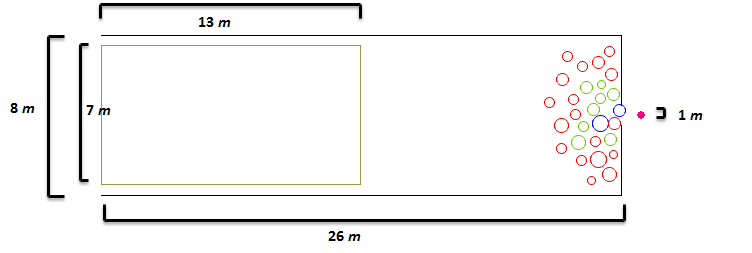
\includegraphics[width=0.8\columnwidth]{figs/scenario_uniflow_individual.png}
\end{center}
\caption{Unidirectional flow simulation for social force model}
\label{fig:scenariouniflow}
\end{figure}
A yellow-start area is designed sufficiently to simulate the maximum population number up to \textit{N} =70  pedestrians (with pedestrian's (\begin{math} \textit{\mu_{radii}}=0.3\; \textit{\sigma_{radii}}=0.05\end{math}). A replication mode is also developed to allow verifying blockage phenomena of each simulation time. 
\section{Escape rate and pedestrian left frequency analysis}
In this experiment, two average cut-off based prototypes are investigated at level 3 (average lv3), and 1 (average lv1). Uniform cut-off based prototypes are also performed at these levels, uniform lv3 and uniform lv1. Parameter distributions of three pedestrian types are sampled 10 times in which each sampling time is simulated 10 times. This work is to investigate different possible parameter values placements of pedestrians in simulation environment. Figures~\ref{interaction_strength_dist} shows parameter distributions at one sampling time on interaction strength \textit{A} parameter. The figure containts parameter distributions of six prototypes including \begin{math} P_{differential}, P_{average}, P_{average\;lv3},\end{math} \begin{math} P_{average\;lv1}, P_{uniform\;lv3}, P_{uniform\;lv1}\end{math} at interaction strength \textit{A} parameter at one sampling time.
\newpage
\begin{figure}[H]
\hspace*{-4cm}   
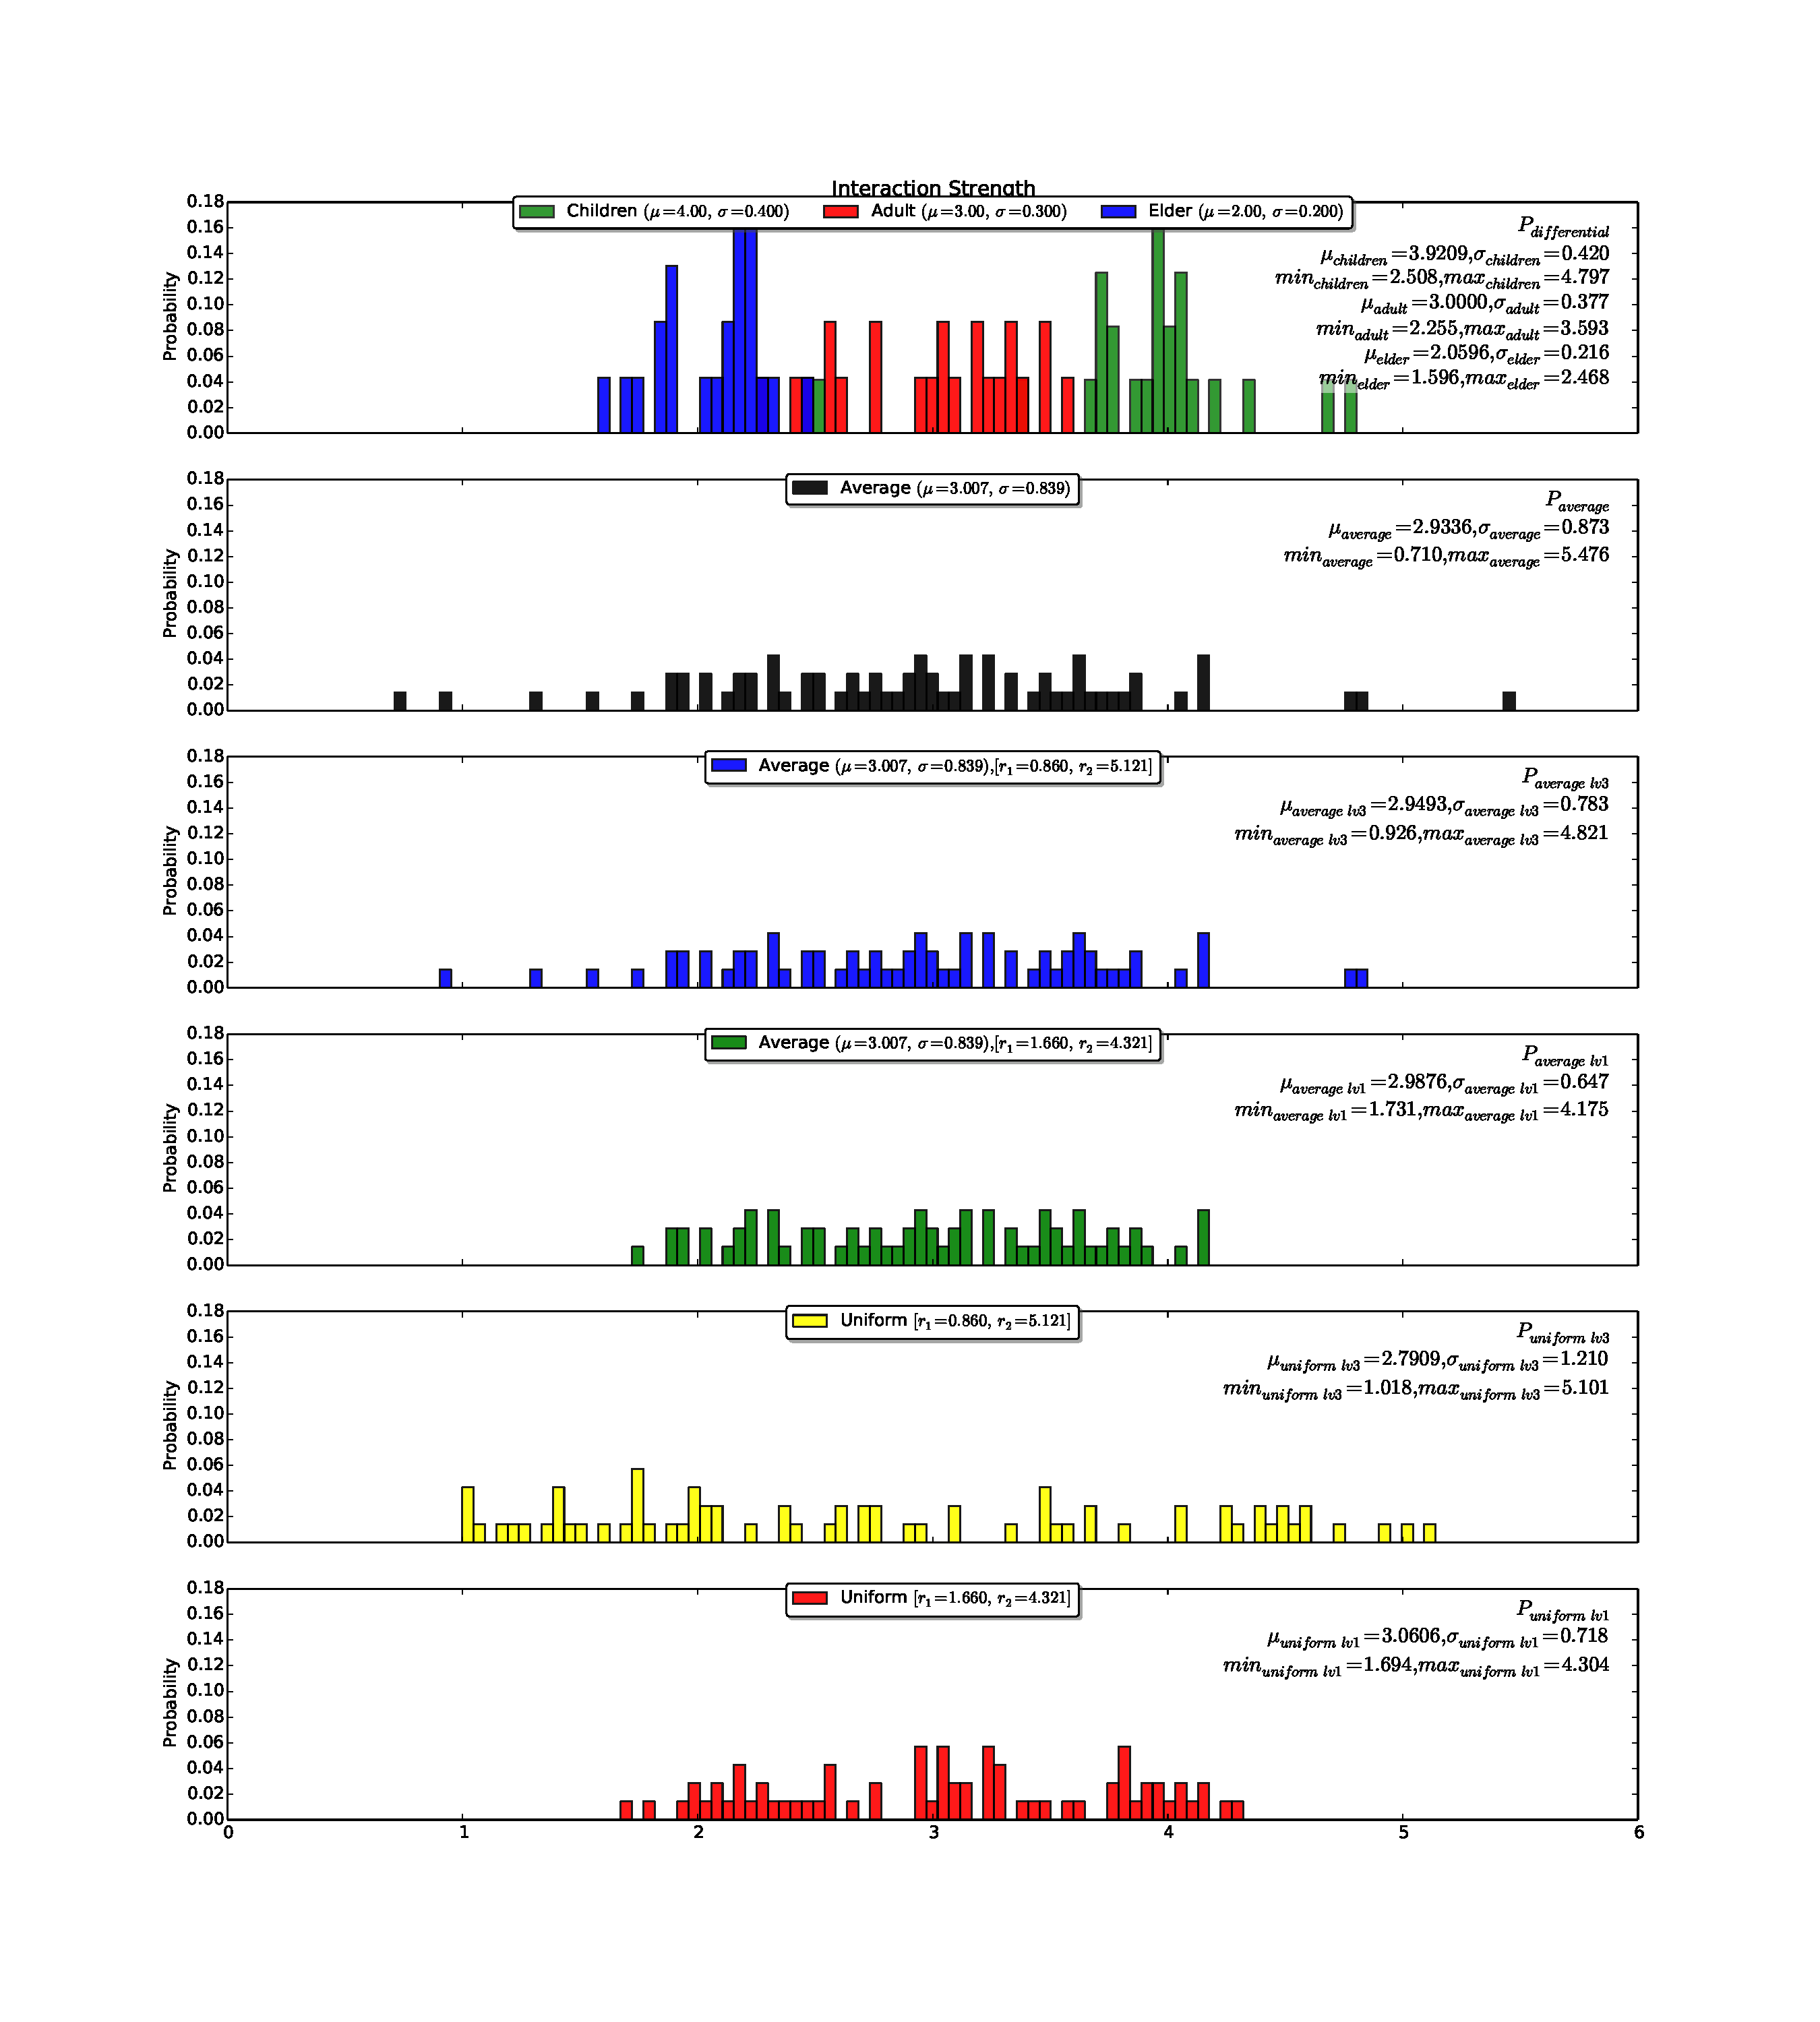
\includegraphics[width=22cm,height=24cm]{figs/interaction_strength_dist.pdf}
\caption{Parameter distributions of six prototypes}
\label{fig:interaction_strength_dist}
\end{figure}
During simulation duration of 100 seconds, escape number and time are monitored. Escape rate is measured by the last escape time of crowd over the total pedestrian have been escaped. This measurement is to remove the influence of counting escape rate by total population number. Figures~\ref{fig:escape_num_dist},~\ref{fig:escape_time_dist}, ~\ref{fig:escape_rate_dist} present escape number, escape time, and escape rates respectively.
\begin{figure}[H]
\begin{center}
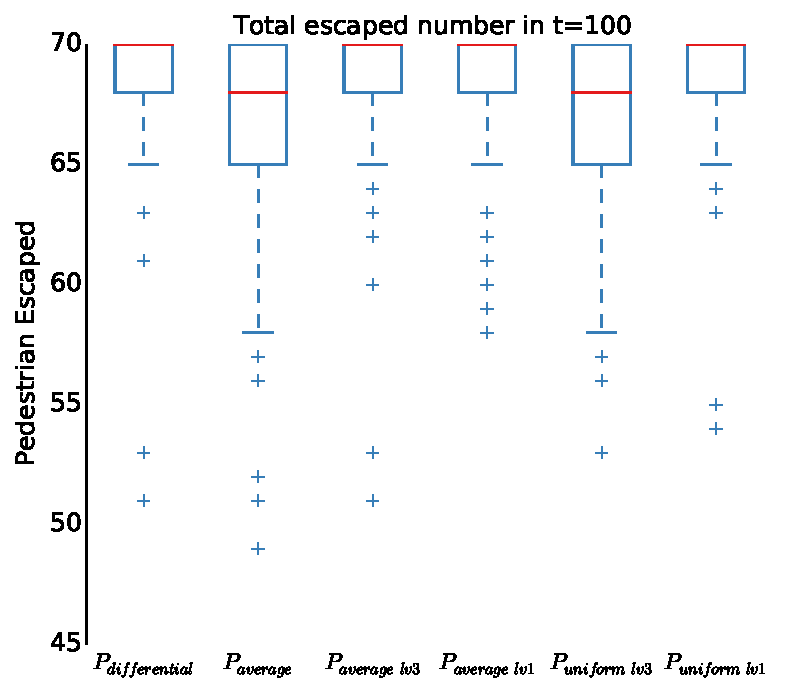
\includegraphics[width=8cm,height=8cm]{figs/escape_number_analysis.pdf}
\end{center}
\caption{Escape number of six prototypes of a population size N = 70}
\label{fig:escape_num_dist}
\end{figure}

\begin{figure}[H]
\begin{center}
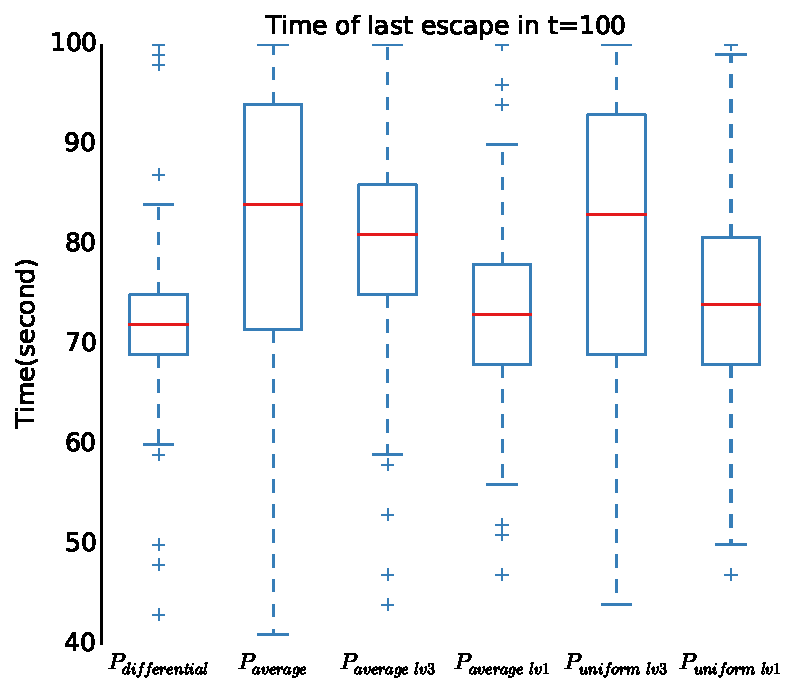
\includegraphics[width=8cm,height=8cm]{figs/escape_time_analysis.pdf}
\end{center}
\caption{Escape time of six prototypes of a population size N = 70}
\label{fig:escape_time_dist}
\end{figure}

\begin{figure}[H]
\begin{center}
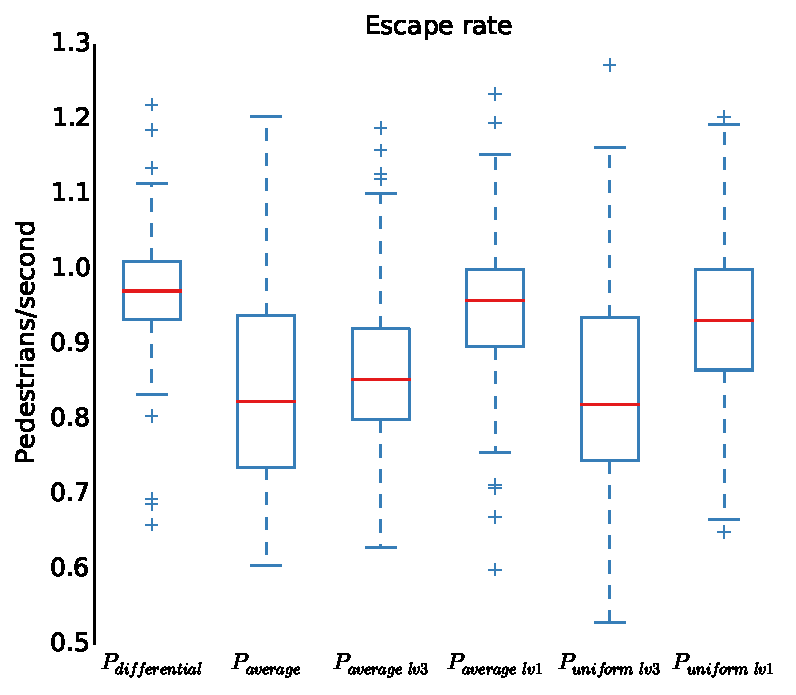
\includegraphics[width=8cm,height=8cm]{figs/escape_rate_analysis.pdf}
\end{center}
\caption{Escape rates of six prototypes of a population size N = 70}
\label{fig:escape_rate_dist}
\end{figure}

Through the observation, the \begin{math} \textit{Prototype_{differential}} \end{math}, which uses different parameter distributions for pedestrian types, generates highest escape rates comparing to other prototypes. Moreover, average-based prototypes have higher escape rate than uniform-based prototypes. Figure~\ref{fig:blockage_frequency} presents pedestrian left frequencies of this experiment.
\begin{figure}[H]
\begin{center}
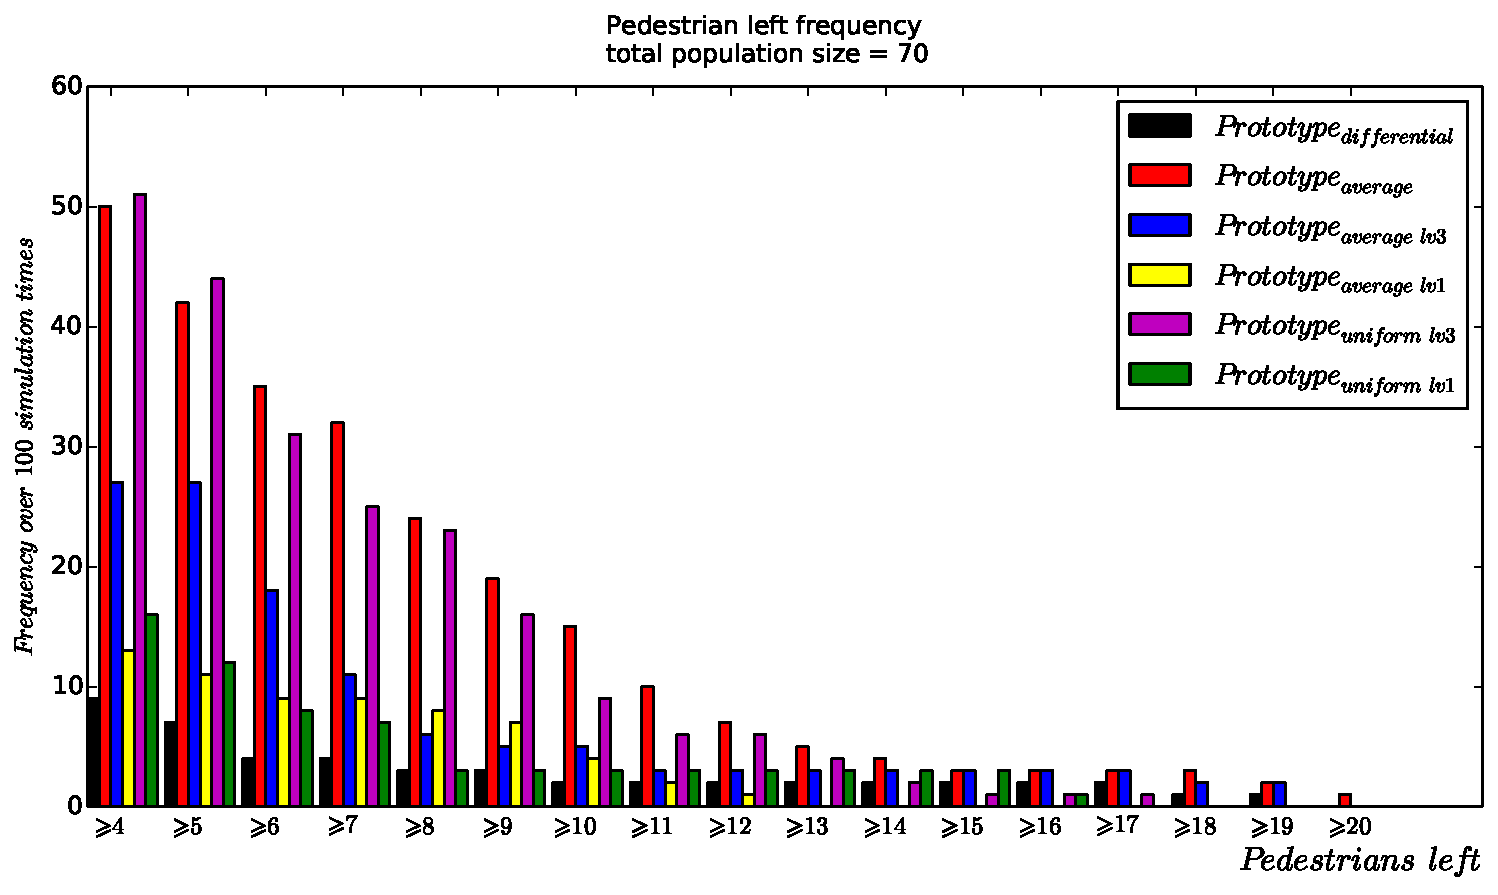
\includegraphics[width=15cm,height=10cm]{figs/blockage_frequency_accumulated_chart.pdf}
\end{center}
\caption{Pedestrian left frequency of six prototypes of the population size N= 70}
\label{fig:blockage_frequency}
\end{figure}
%%%%%%%%%%%%%%%%%%%%%%%%%%%%%%%%%%%%%%%%%%%%%%%%%%%%%%%%%%%%%%%%%%%%%%%%%%%%%%
%%
%% Back matter 
%%

\backmatter% start the thesis back matter
\bibliographystyle{apacite}
\bibliography{confirmationmonashbib}
\end{document}
